\documentclass[12pt]{article}
\usepackage[utf8]{inputenc}
\usepackage{amsmath,amsthm,amsfonts,amssymb}
\usepackage{tikz}
\usepackage{subfig}
\usepackage[english]{babel}
\usepackage{capt-of}
\newtheorem{theorem}{Theorem}
\usetikzlibrary{calc}
\usetikzlibrary{shapes}
\usepackage{hyperref}
%might be unnecessary
\usepackage{doi}

%bibliography CMDS

%\usepackage{cite}
%\usepackage[style=alphabetic]{biblatex}
%\bibliographystyle{plain}

%\usepackage[style=alphabetic]{biblatex}

% \usepackage[backend=biber,style=alphabetic]{biblatex}
\usepackage[backend=biber,style=numeric]{biblatex}
% \usepackage[backend=biber,style=abbrv]{biblatex}
% \usepackage[backend=biber,style=alpha]{biblatex}
%\usepackage[backend=bibtex,style=alphabetic]{biblatex}
\addbibresource{./bibb.bib}

%%% With amsthm package, creates environments for nicely formatted,
%%% labeled, and numbered propositions, etc.
\theoremstyle{plain}
\newtheorem{thm}{Theorem}
\newtheorem{lemma}[thm]{Lemma}
\newtheorem{prop}[thm]{Proposition}
\newtheorem{conj}[thm]{Conjecture}
\newtheorem{cor}[thm]{Corollary}
\newtheorem{claim}[thm]{Claim}
\newtheorem{fact}[thm]{Fact}
\newtheorem{constraint}[thm]{Constraint}

\theoremstyle{definition}
\newtheorem{eg}[thm]{Example}
\newtheorem{defn}[thm]{Definition}
\newtheorem{rem}[thm]{Remark}
\newtheorem{observ}[thm]{Observation}
\newtheorem{open}[thm]{Open Problem}
\newtheorem{prob.}[thm]{Problem}
\newtheorem{quest}[thm]{Question}

% I used these for making definitions and theorems, not what is above
\theoremstyle{remark}
\newtheorem{remark}[thm]{Remark}
\newtheorem{note}[thm]{Note}
\theoremstyle{definition}
\newtheorem{definition}{Definition}[section]
\newtheorem{exmp}{Example}[section]

%custom commands

% blank cell
\newcommand{\cell}[4]{ \draw[thick] ( #1 , #2 ) rectangle ( #3 , #4 );}

% open cell 
\newcommand{\cellopen}[4]{ \draw[thick] ( #1 , #2 ) rectangle ( #3 , #4 ); \node[shape=circle,draw=red,fill=red, inner sep=0pt,minimum size=3pt] (A) at ( #1 * 0.5 + #3 * 0.5 , #2 * 0.5 + #4 * 0.5 ){};}

% /
\newcommand{\cellA}[4]{ \draw[thick] ( #1 , #2 ) rectangle ( #3 , #4 ); \draw[red, thick, densely dotted] (#3 * 0.5 + #1 * 0.5 , #2) -- (#3, #4 * 0.5 + #2 * 0.5);}

% \
\newcommand{\cellB}[4]{ \draw[thick] ( #1 , #2 ) rectangle ( #3 , #4 ); \draw[red, thick, densely dotted] (#3 * 0.5 + #1 * 0.5 , #2) -- (#1, #4 * 0.5 + #2 * 0.5);}

% /
\newcommand{\cellC}[4]{ \draw[thick] ( #1 , #2 ) rectangle ( #3 , #4 ); \draw[red, thick, densely dotted] (#3 * 0.5 + #1 * 0.5 , #4) -- (#1, #4 * 0.5 + #2 * 0.5);}

% L
\newcommand{\cellD}[4]{ \draw[thick] ( #1 , #2 ) rectangle ( #3 , #4 ); \draw[red, thick, densely dotted] (#3 * 0.5 + #1 * 0.5 , #4) -- (#3, #4 * 0.5 + #2 * 0.5);}

% |
\newcommand{\cellE}[4]{ \draw[thick] ( #1 , #2 ) rectangle ( #3 , #4 ); \draw[red, thick, densely dotted] (#3 * 0.5 + #1 * 0.5 , #2) -- (#3 * 0.5 + #1 * 0.5 , #4);}

% -
\newcommand{\cellF}[4]{ \draw[thick] ( #1 , #2 ) rectangle ( #3 , #4 ); \draw[red, thick, densely dotted] (#3, #4 * 0.5 + #2 * 0.5) -- (#1, #4 * 0.5 + #2 * 0.5);}

\newcommand{\cellAf}[4]{\filldraw[gray!40] ( #1 , #2 ) rectangle ( #3 , #4 ); \draw[thick] ( #1 , #2 ) rectangle ( #3 , #4 ); \draw[red, thick, densely dotted] (#3 * 0.5 + #1 * 0.5 , #2) -- (#3, #4 * 0.5 + #2 * 0.5);}

% \
\newcommand{\cellBf}[4]{\filldraw[gray!40] ( #1 , #2 ) rectangle ( #3 , #4 ); \draw[thick] ( #1 , #2 ) rectangle ( #3 , #4 ); \draw[red, thick, densely dotted] (#3 * 0.5 + #1 * 0.5 , #2) -- (#1, #4 * 0.5 + #2 * 0.5);}

% /
\newcommand{\cellCf}[4]{\filldraw[gray!40] ( #1 , #2 ) rectangle ( #3 , #4 ); \draw[thick] ( #1 , #2 ) rectangle ( #3 , #4 ); \draw[red, thick, densely dotted] (#3 * 0.5 + #1 * 0.5 , #4) -- (#1, #4 * 0.5 + #2 * 0.5);}

% L
\newcommand{\cellDf}[4]{\filldraw[gray!40] ( #1 , #2 ) rectangle ( #3 , #4 ); \draw[thick] ( #1 , #2 ) rectangle ( #3 , #4 ); \draw[red, thick, densely dotted] (#3 * 0.5 + #1 * 0.5 , #4) -- (#3, #4 * 0.5 + #2 * 0.5);}

% |
\newcommand{\cellEf}[4]{\filldraw[gray!40] ( #1 , #2 ) rectangle ( #3 , #4 ); \draw[thick] ( #1 , #2 ) rectangle ( #3 , #4 ); \draw[red, thick, densely dotted] (#3 * 0.5 + #1 * 0.5 , #2) -- (#3 * 0.5 + #1 * 0.5 , #4);}

% -
\newcommand{\cellFf}[4]{\filldraw[gray!40] ( #1 , #2 ) rectangle ( #3 , #4 ); \draw[thick] ( #1 , #2 ) rectangle ( #3 , #4 ); \draw[red, thick, densely dotted] (#3, #4 * 0.5 + #2 * 0.5) -- (#1, #4 * 0.5 + #2 * 0.5);}


\newcommand{\lablnode}[3]{\node[shape=circle,draw=none,fill=none, inner sep=0pt,minimum size=0pt] (A) at ( #1 , #2 ) {#3};}

\usepackage[margin=1in]{geometry}
\date{}
%doc info
% $\text{Hanke, Jack}^*$\\
% $\text{Schank, Richard}$\\
% $\text{Maltenfort, Michael}^*$
\author{
    \textbf{Jack Hanke}\\
    Northwestern University
    \and
    \textbf{Richard Schank}\\
    \and
    \textbf{Michael Maltenfort}\\
    Northwestern University
    }
\title{\textbf{Exact Enumeration of Polygon Mosaics}}
% \date{\today}

\begin{document}
\maketitle

\begin{center}

    \begin{abstract}
        Hong and Oh calculated upper and lower bounds on the number of polygon mosaics for $7$ distinct tiles that together model multiple ring polymers in physics. We exactly enumerate these polygon mosaics. The method we introduce generalizes to various other tile sets. We also introduce and enumerate a variation on polygon mosaics called messy polygon mosaics for various tile sets.
    \end{abstract}

\end{center}

\section{Introduction}

Consider the following set of $7$ symbols labelled $\{ T_1, \dots T_7 \}$ composed of unit squares and dotted lines connecting pairs of sides at their midpoints.

\begin{center}
    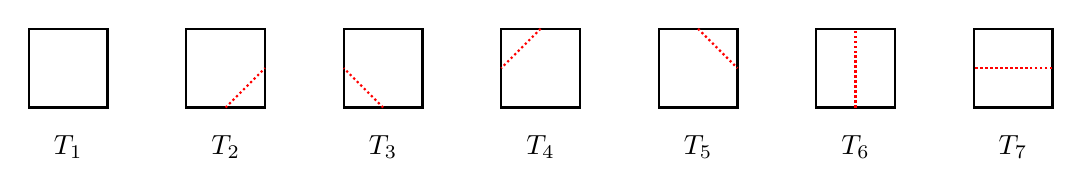
\begin{tikzpicture}
        \cell{-2}{0}{-1}{1}
        \( \lablnode{-1.5}{-0.5}{$T_1$} \) 
        \cellA{0}{0}{1}{1}
        \( \lablnode{0.5}{-0.5}{$T_2$} \) 
        \cellB{2}{0}{3}{1}
        \( \lablnode{2.5}{-0.5}{$T_3$} \) 
        \cellC{4}{0}{5}{1}
        \( \lablnode{4.5}{-0.5}{$T_4$} \) 
        \cellD{6}{0}{7}{1}
        \( \lablnode{6.5}{-0.5}{$T_5$} \) 
        \cellE{8}{0}{9}{1}
        \( \lablnode{8.5}{-0.5}{$T_6$} \) 
        \cellF{10}{0}{11}{1}
        \( \lablnode{10.5}{-0.5}{$T_7$} \) 
    \end{tikzpicture}
\end{center}

Call these symbols \textit{tiles}. A \textit{mosaic} of size $(n, m)$ is an $n \times m$ matrix of these tiles. For example, below is a mosaic of size $(5,7)$.

\begin{center}
    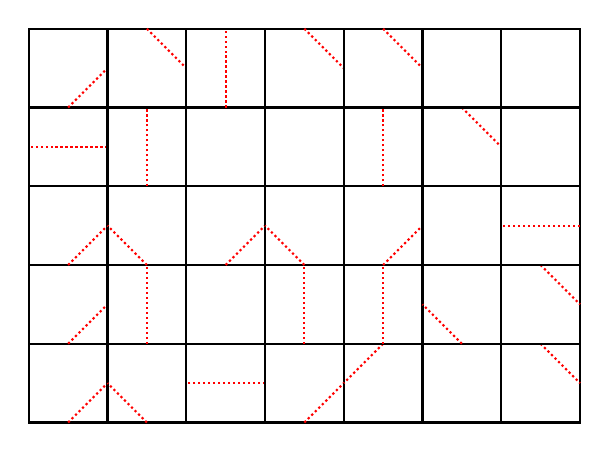
\begin{tikzpicture}
        % row1
        \cellA{0}{0}{1}{1}
        \cellB{1}{0}{2}{1}
        \cellF{2}{0}{3}{1}
        \cellA{3}{0}{4}{1}
        \cellC{4}{0}{5}{1}
        \cell{5}{0}{6}{1}
        \cellD{6}{0}{7}{1}
        % row2
        \cellA{0}{1}{1}{2}
        \cellE{1}{1}{2}{2}
        \cell{2}{1}{3}{2}
        \cellE{3}{1}{4}{2}
        \cellE{4}{1}{5}{2}
        \cellB{5}{1}{6}{2}
        \cellD{6}{1}{7}{2}
        % row3
        \cellA{0}{2}{1}{3}
        \cellB{1}{2}{2}{3}
        \cellA{2}{2}{3}{3}
        \cellB{3}{2}{4}{3}
        \cellA{4}{2}{5}{3}
        \cell{5}{2}{6}{3}
        \cellF{6}{2}{7}{3}
        % row4
        \cellF{0}{3}{1}{4}
        \cellE{1}{3}{2}{4}
        \cell{2}{3}{3}{4}
        \cell{3}{3}{4}{4}
        \cellE{4}{3}{5}{4}
        \cellD{5}{3}{6}{4}
        \cell{6}{3}{7}{4}
        % row5
        \cellA{0}{4}{1}{5}
        \cellD{1}{4}{2}{5}
        \cellE{2}{4}{3}{5}
        \cellD{3}{4}{4}{5}
        \cellD{4}{4}{5}{5}
        \cell{5}{4}{6}{5}
        \cell{6}{4}{7}{5}
\end{tikzpicture}
\end{center}

Consider a shared edge between two tiles in the above figure. The edge has either $0$, $1$, or $2$ dotted lines drawn from its midpoint. Also note that the edges of the tiles on the boundary of the matrix are not shared by another tile. Therefore these edges only have $0$ or $1$ dotted lines drawn from their midpoint. We define a \textit{polygon mosaic} to be a mosaic that has all shared edges between tiles having $0$ or $2$ dotted lines drawn from their midpoint, and $0$ dotted lines drawn from the boundary edges. 

We call these polygon mosaics because, other than the mosaic consisting of all $T_1$ tiles, the dotted lines form shapes we call \textit{polygons}. 

\begin{exmp}
\label{exmp: clean sap}
Below is an example of a polygon mosaic of size $(5,7)$ that contains $2$ polygons, hilighted in gray.

\begin{center}
    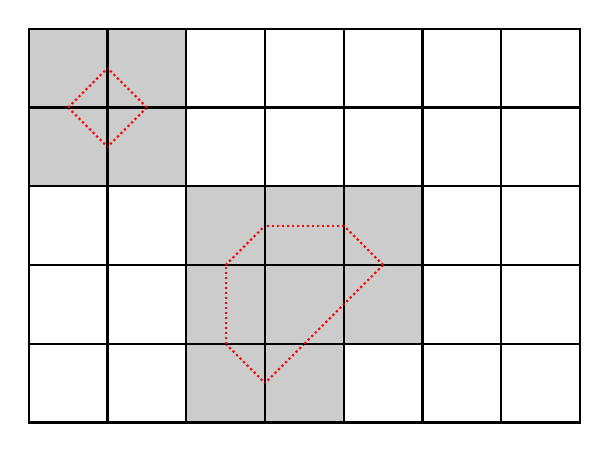
\begin{tikzpicture}
        % row1
        \cell{0}{0}{1}{1}
        \cell{1}{0}{2}{1}
        \cellDf{2}{0}{3}{1}
        \cellCf{3}{0}{4}{1}
        \cell{4}{0}{5}{1}
        \cell{5}{0}{6}{1}
        \cell{6}{0}{7}{1}
        % row2
        \cell{0}{1}{1}{2}
        \cell{1}{1}{2}{2}
        \cellEf{2}{1}{3}{2}
        \cellAf{3}{1}{4}{2}
        \cellCf{4}{1}{5}{2}
        \cell{5}{1}{6}{2}
        \cell{6}{1}{7}{2}
        % row3
        \cell{0}{2}{1}{3}
        \cell{1}{2}{2}{3}
        \cellAf{2}{2}{3}{3}
        \cellFf{3}{2}{4}{3}
        \cellBf{4}{2}{5}{3}
        \cell{5}{2}{6}{3}
        \cell{6}{2}{7}{3}
        % row4
        \cellDf{0}{3}{1}{4}
        \cellCf{1}{3}{2}{4}
        \cell{2}{3}{3}{4}
        \cell{3}{3}{4}{4}
        \cell{4}{3}{5}{4}
        \cell{5}{3}{6}{4}
        \cell{6}{3}{7}{4}
        % row5
        \cellAf{0}{4}{1}{5}
        \cellBf{1}{4}{2}{5}
        \cell{2}{4}{3}{5}
        \cell{3}{4}{4}{5}
        \cell{4}{4}{5}{5}
        \cell{5}{4}{6}{5}
        \cell{6}{4}{7}{5}
    \end{tikzpicture}
\end{center}
\end{exmp}

These polygons \footnote{Polygons are more commonly called "self-avoiding polygons" in the literature to emphasize their relationship with self-avoiding walks.} can be formed with any even number of tiles greater than $2$, and can take on many shapes. In large enough mosaics, larger polygons can surround smaller polygons. 

Let $p_{n,m}$ be the number of polygon mosaics of size $(n,m)$. First notice that if either $n$ or $m$ is $1$, one cannot construct a polygon mosaic, so 
$$p_{n,1} = p_{1,m} = 0.$$

Hong and Oh \cite[Hong2018]{Hong2018} gave the following upper and lower bounds \footnote{The authors did not consider the mosaic containing all $T_1$ tiles a polygon mosaic, and so define $p_{n,m}$ as one less than what we define.} for $n,m \geq 2$. 

$$2^{n+m-3} \left(\frac{17}{10}\right)^{(n-2)(m-2)} \leq p_{n,m} \leq 2^{n+m-3} \left(\frac{31}{16}\right)^{(n-2)(m-2)}.$$

We give an exact expression for $p_{n,m}$ for $n,m \geq 2$ in Theorem \ref{thm: main theorem}. We also introduce and enumerate \textit{messy polygon mosaics}, a variant on the previously studied polygon mosaics with a similar enumeration strategy.

\begin{thm}
\label{thm: main theorem}

To enumerate $p_{n,m}$, we construct $A(m) \in \mathbb{Z}^{2^{m-1} \times 2^{m-1}}$ recursively with the initial matrix $
A(2) = \begin{bmatrix}
1 & 1 \\
1 & 1
\end{bmatrix}
$. We recursively define $A(k+1)$ given $A(k)$. Begin by writing
$
A(k) = \begin{bmatrix}
A_1 & A_2 \\
A_3 & A_4
\end{bmatrix}
$, where the block matrices $A_i$ are square block matrices of size $2^{m-2} \times 2^{m-2}$, or scalars if $m=2$. Then we have

$$
A(k+1) = \begin{bmatrix}
A_1 & A_2 & A_1 & A_2 \\
A_3 & A_4 & 0A_3 & A_4 \\
A_1 & 0A_2 & A_1 & A_2 \\
A_3 & A_4 & A_3 & A_4 \\
\end{bmatrix},
$$

where products of a scalar and block matrix are done element-wise. Construct $A(m)$ by starting with $k=2$ and recursing until $k=m$. Next denote the rows and columns of $A(m)$ as
$$
A(m) = 
\begin{bmatrix}
    r_1 \\
    r_2 \\
    ... \\
    r_{2^{m-1}} \\
\end{bmatrix} = 
\begin{bmatrix}
    c_1 & c_2 & ... & c_{2^{m-1}}
\end{bmatrix}
$$

Then $p_{n,m} = r_1 A(m)^{n-2}c_1 .$
\end{thm}

\section{Proof of Theorem \ref{thm: main theorem}}

\begin{proof}

For a given mosaic, color the vertices of the tiles as follows. If the vertex is surrounded by an even number of polygons, color it black. If the vertex is surrounded by an odd number of polygons, color it white with a green border. To make a \textit{vertex coloring} we also remove the dotted lines from all tiles in the mosaic. 

Using the mosaic from Example \ref{exmp: clean sap}, we show both the coloring of the mosaic, and then the removal of the dotted lines.

\begin{center}
    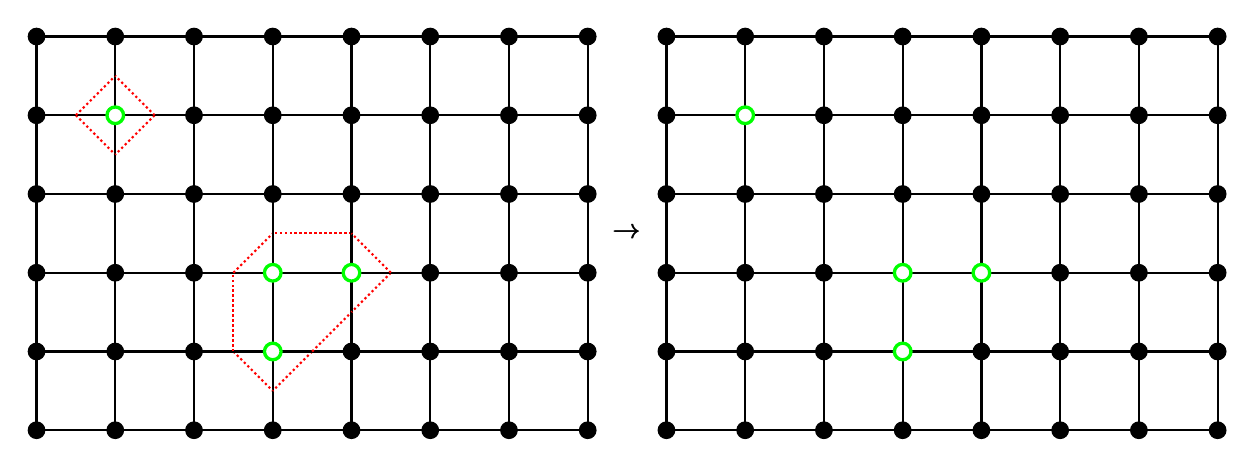
\begin{tikzpicture}
        % row1
        \cell{0}{0}{1}{1}
        \cell{1}{0}{2}{1}
        \cellD{2}{0}{3}{1}
        \cellC{3}{0}{4}{1}
        \cell{4}{0}{5}{1}
        \cell{5}{0}{6}{1}
        \cell{6}{0}{7}{1}
        % row2
        \cell{0}{1}{1}{2}
        \cell{1}{1}{2}{2}
        \cellE{2}{1}{3}{2}
        \cellA{3}{1}{4}{2}
        \cellC{4}{1}{5}{2}
        \cell{5}{1}{6}{2}
        \cell{6}{1}{7}{2}
        % row3
        \cell{0}{2}{1}{3}
        \cell{1}{2}{2}{3}
        \cellA{2}{2}{3}{3}
        \cellF{3}{2}{4}{3}
        \cellB{4}{2}{5}{3}
        \cell{5}{2}{6}{3}
        \cell{6}{2}{7}{3}
        % row4
        \cellD{0}{3}{1}{4}
        \cellC{1}{3}{2}{4}
        \cell{2}{3}{3}{4}
        \cell{3}{3}{4}{4}
        \cell{4}{3}{5}{4}
        \cell{5}{3}{6}{4}
        \cell{6}{3}{7}{4}
        % row5
        \cellA{0}{4}{1}{5}
        \cellB{1}{4}{2}{5}
        \cell{2}{4}{3}{5}
        \cell{3}{4}{4}{5}
        \cell{4}{4}{5}{5}
        \cell{5}{4}{6}{5}
        \cell{6}{4}{7}{5}
        % label for row1
        \draw[fill=black] (0,0) circle (3pt);
        \draw[fill=black] (1,0) circle (3pt);
        \draw[fill=black] (2,0) circle (3pt);
        \draw[fill=black] (3,0) circle (3pt);
        \draw[fill=black] (4,0) circle (3pt);
        \draw[fill=black] (5,0) circle (3pt);
        \draw[fill=black] (6,0) circle (3pt);
        \draw[fill=black] (7,0) circle (3pt);
        % label for row1
        \draw[fill=black] (0,1) circle (3pt);
        \draw[fill=black] (1,1) circle (3pt);
        \draw[fill=black] (2,1) circle (3pt);
        \draw[fill=white, draw=green, very thick] (3,1) circle (3pt);
        \draw[fill=black] (4,1) circle (3pt);
        \draw[fill=black] (5,1) circle (3pt);
        \draw[fill=black] (6,1) circle (3pt);
        \draw[fill=black] (7,1) circle (3pt);
        % label for row1
        \draw[fill=black] (0,2) circle (3pt);
        \draw[fill=black] (1,2) circle (3pt);
        \draw[fill=black] (2,2) circle (3pt);
        \draw[fill=white, draw=green, very thick] (3,2) circle (3pt);
        \draw[fill=white, draw=green, very thick] (4,2) circle (3pt);
        \draw[fill=black] (5,2) circle (3pt);
        \draw[fill=black] (6,2) circle (3pt);
        \draw[fill=black] (7,2) circle (3pt);
        % label for row1
        \draw[fill=black] (0,3) circle (3pt);
        \draw[fill=black] (1,3) circle (3pt);
        \draw[fill=black] (2,3) circle (3pt);
        \draw[fill=black] (3,3) circle (3pt);
        \draw[fill=black] (4,3) circle (3pt);
        \draw[fill=black] (5,3) circle (3pt);
        \draw[fill=black] (6,3) circle (3pt);
        \draw[fill=black] (7,3) circle (3pt);
        % label for row1
        \draw[fill=black] (0,4) circle (3pt);
        \draw[fill=white, draw=green, very thick] (1,4) circle (3pt);
        \draw[fill=black] (2,4) circle (3pt);
        \draw[fill=black] (3,4) circle (3pt);
        \draw[fill=black] (4,4) circle (3pt);
        \draw[fill=black] (5,4) circle (3pt);
        \draw[fill=black] (6,4) circle (3pt);
        \draw[fill=black] (7,4) circle (3pt);
        % label for row1
        \draw[fill=black] (0,5) circle (3pt);
        \draw[fill=black] (1,5) circle (3pt);
        \draw[fill=black] (2,5) circle (3pt);
        \draw[fill=black] (3,5) circle (3pt);
        \draw[fill=black] (4,5) circle (3pt);
        \draw[fill=black] (5,5) circle (3pt);
        \draw[fill=black] (6,5) circle (3pt);
        \draw[fill=black] (7,5) circle (3pt);

        % arrow
        \( \lablnode{7.5}{2.5}{$\pmb{\to}$} \)        

        % row1
        \cell{8}{0}{9}{1}
        \cell{9}{0}{10}{1}
        \cell{10}{0}{11}{1}
        \cell{11}{0}{12}{1}
        \cell{12}{0}{13}{1}
        \cell{13}{0}{14}{1}
        \cell{14}{0}{15}{1}
        % row2
        \cell{8}{1}{9}{2}
        \cell{9}{1}{10}{2}
        \cell{10}{1}{11}{2}
        \cell{11}{1}{12}{2}
        \cell{12}{1}{13}{2}
        \cell{13}{1}{14}{2}
        \cell{14}{1}{15}{2}
        % row3
        \cell{8}{2}{9}{3}
        \cell{9}{2}{10}{3}
        \cell{10}{2}{11}{3}
        \cell{11}{2}{12}{3}
        \cell{12}{2}{13}{3}
        \cell{13}{2}{14}{3}
        \cell{14}{2}{15}{3}
        % row4
        \cell{8}{3}{9}{4}
        \cell{9}{3}{10}{4}
        \cell{10}{3}{11}{4}
        \cell{11}{3}{12}{4}
        \cell{12}{3}{13}{4}
        \cell{13}{3}{14}{4}
        \cell{14}{3}{15}{4}
        % row5
        \cell{8}{4}{9}{5}
        \cell{9}{4}{10}{5}
        \cell{10}{4}{11}{5}
        \cell{11}{4}{12}{5}
        \cell{12}{4}{13}{5}
        \cell{13}{4}{14}{5}
        \cell{14}{4}{15}{5}
        % label for row1
        \draw[fill=black] (8,0) circle (3pt);
        \draw[fill=black] (9,0) circle (3pt);
        \draw[fill=black] (10,0) circle (3pt);
        \draw[fill=black] (11,0) circle (3pt);
        \draw[fill=black] (12,0) circle (3pt);
        \draw[fill=black] (13,0) circle (3pt);
        \draw[fill=black] (14,0) circle (3pt);
        \draw[fill=black] (15,0) circle (3pt);
        % label for row1
        \draw[fill=black] (8,1) circle (3pt);
        \draw[fill=black] (9,1) circle (3pt);
        \draw[fill=black] (10,1) circle (3pt);
        \draw[fill=white, draw=green, very thick] (11,1) circle (3pt);
        \draw[fill=black] (12,1) circle (3pt);
        \draw[fill=black] (13,1) circle (3pt);
        \draw[fill=black] (14,1) circle (3pt);
        \draw[fill=black] (15,1) circle (3pt);
        % label for row1
        \draw[fill=black] (8,2) circle (3pt);
        \draw[fill=black] (9,2) circle (3pt);
        \draw[fill=black] (10,2) circle (3pt);
        \draw[fill=white, draw=green, very thick] (11,2) circle (3pt);
        \draw[fill=white, draw=green, very thick] (12,2) circle (3pt);
        \draw[fill=black] (13,2) circle (3pt);
        \draw[fill=black] (14,2) circle (3pt);
        \draw[fill=black] (15,2) circle (3pt);
        % label for row1
        \draw[fill=black] (8,3) circle (3pt);
        \draw[fill=black] (9,3) circle (3pt);
        \draw[fill=black] (10,3) circle (3pt);
        \draw[fill=black] (11,3) circle (3pt);
        \draw[fill=black] (12,3) circle (3pt);
        \draw[fill=black] (13,3) circle (3pt);
        \draw[fill=black] (14,3) circle (3pt);
        \draw[fill=black] (15,3) circle (3pt);
        % label for row1
        \draw[fill=black] (8,4) circle (3pt);
        \draw[fill=white, draw=green, very thick] (9,4) circle (3pt);
        \draw[fill=black] (10,4) circle (3pt);
        \draw[fill=black] (11,4) circle (3pt);
        \draw[fill=black] (12,4) circle (3pt);
        \draw[fill=black] (13,4) circle (3pt);
        \draw[fill=black] (14,4) circle (3pt);
        \draw[fill=black] (15,4) circle (3pt);
        % label for row1
        \draw[fill=black] (8,5) circle (3pt);
        \draw[fill=black] (9,5) circle (3pt);
        \draw[fill=black] (10,5) circle (3pt);
        \draw[fill=black] (11,5) circle (3pt);
        \draw[fill=black] (12,5) circle (3pt);
        \draw[fill=black] (13,5) circle (3pt);
        \draw[fill=black] (14,5) circle (3pt);
        \draw[fill=black] (15,5) circle (3pt);
    \end{tikzpicture}
\end{center}

The critical point is this: even with the dotted lines removed, the vertex coloring uniquely identifies the polygon mosaic. This is true even if there are polygons surrounding other polygons. We can then enumerate $p_{n,m}$ by enumerating the number of vertex colorings that correspond with a valid polygon mosaic. 

Consider the collection of vertex colorings. Each boundary vertex is necessarily colored black, and each interior vertex is colored either black or white with a green border. Of these $2^{(n-1)(m-1)}$ colorings, the colorings that correspond with valid polygon mosaics are ones that do not contain the following two sub-colorings.

\begin{center}
    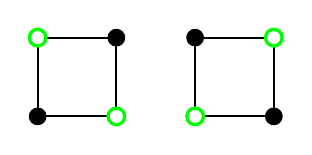
\begin{tikzpicture}
        % row1
        \cell{0}{0}{1}{1}
        \cell{2}{0}{3}{1}

        \draw[fill=black] (0,0) circle (3pt);
        \draw[fill=white, draw=green, very thick] (1,0) circle (3pt);
        \draw[fill=white, draw=green, very thick] (2,0) circle (3pt);
        \draw[fill=black] (3,0) circle (3pt);

        \draw[fill=white, draw=green, very thick] (0,1) circle (3pt);
        \draw[fill=black] (1,1) circle (3pt);
        \draw[fill=black] (2,1) circle (3pt);
        \draw[fill=white, draw=green, very thick] (3,1) circle (3pt);
        
    \end{tikzpicture}
\end{center}

These two sub-colorings aren't associasted with any of our tiles $T_1, \dots, T_7$, and so cannot possibly be created from the coloring process. 

We seek a recursive solution to enumerate the number of vertex colorings that avoid these sub-colorings. We start with a $n \times 1$ matrix for fixed $n$. We intend to build vertex colorings of an $n \times m$ matrix, so the upper and lower boundary vertices are colored black. We also build these matrices from right to left, so the right boundary vertices is also black. We have no conditions on the boundary of the left vertices, and so there are $2^{n-1}$ initial conditions. One of these initial conditions is below.

\begin{center}
    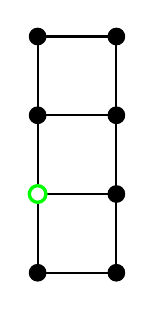
\begin{tikzpicture}
        \cell{0}{0}{1}{1}
        \cell{0}{1}{1}{2}
        \cell{0}{2}{1}{3}

        % row 1
        \draw[fill=black] (0,0) circle (3pt);
        \draw[fill=white, draw=green, very thick] (0,1) circle (3pt);
        \draw[fill=black] (0,2) circle (3pt);
        \draw[fill=black] (0,3) circle (3pt);

        \draw[fill=black] (1,0) circle (3pt);
        \draw[fill=black] (1,1) circle (3pt);
        \draw[fill=black] (1,2) circle (3pt);
        \draw[fill=black] (1,3) circle (3pt);
    \end{tikzpicture}
\end{center}

If we append some new column of vertex colorings to the left, the newly created $n \times 2$ matrix may or may not have created an illegal sub-coloring. In the below example, the new left column does not create an illegal sub-coloring.  

\begin{center}
    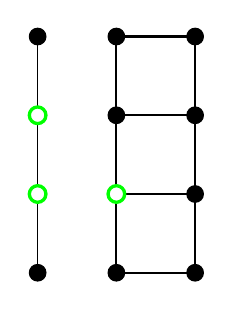
\begin{tikzpicture}
        \cell{0}{0}{1}{1}
        \cell{0}{1}{1}{2}
        \cell{0}{2}{1}{3}

        \draw[black] (-1,0) -- (-1,3);
        % row 1
        \draw[fill=black] (-1,0) circle (3pt);
        \draw[fill=white, draw=green, very thick] (-1,1) circle (3pt);
        \draw[fill=white, draw=green, very thick] (-1,2) circle (3pt);
        \draw[fill=black] (-1,3) circle (3pt);

        \draw[fill=black] (0,0) circle (3pt);
        \draw[fill=white, draw=green, very thick] (0,1) circle (3pt);
        \draw[fill=black] (0,2) circle (3pt);
        \draw[fill=black] (0,3) circle (3pt);

        \draw[fill=black] (1,0) circle (3pt);
        \draw[fill=black] (1,1) circle (3pt);
        \draw[fill=black] (1,2) circle (3pt);
        \draw[fill=black] (1,3) circle (3pt);
    \end{tikzpicture}
\end{center}

With this in mind, we can create a transition matrix that maps every right edge vertex coloring to every left edge vertex coloring, and assigns the value of $0$ to $n\times1$ columns that contain illegal colorings, and $1$ otherwise.  Below is a diagram for the $n=3$ matrix. 

\begin{center}
    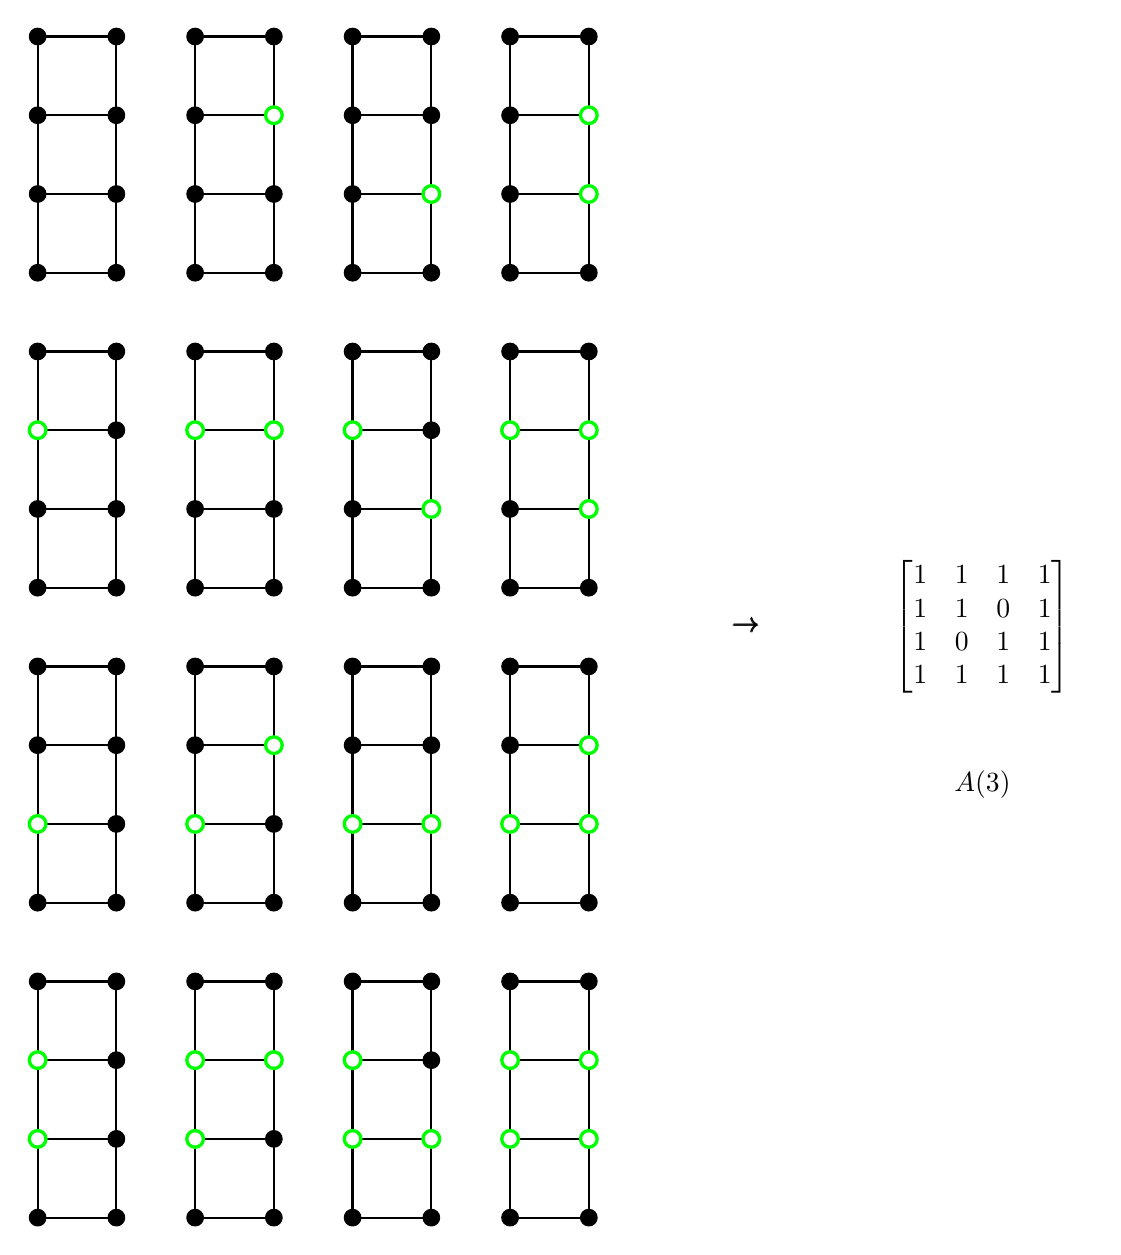
\begin{tikzpicture}
        % row1
        \cell{0}{0}{1}{1}
        \cell{0}{1}{1}{2}
        \cell{0}{2}{1}{3}

        \cell{2}{0}{3}{1}
        \cell{2}{1}{3}{2}
        \cell{2}{2}{3}{3}

        \cell{4}{0}{5}{1}
        \cell{4}{1}{5}{2}
        \cell{4}{2}{5}{3}

        \cell{6}{0}{7}{1}
        \cell{6}{1}{7}{2}
        \cell{6}{2}{7}{3}
        % row2
        \cell{0}{4}{1}{5}
        \cell{0}{5}{1}{6}
        \cell{0}{6}{1}{7}

        \cell{2}{4}{3}{5}
        \cell{2}{5}{3}{6}
        \cell{2}{6}{3}{7}

        \cell{4}{4}{5}{5}
        \cell{4}{5}{5}{6}
        \cell{4}{6}{5}{7}

        \cell{6}{4}{7}{5}
        \cell{6}{5}{7}{6}
        \cell{6}{6}{7}{7}
        % row3
        \cell{0}{8}{1}{9}
        \cell{0}{9}{1}{10}
        \cell{0}{10}{1}{11}

        \cell{2}{8}{3}{9}
        \cell{2}{9}{3}{10}
        \cell{2}{10}{3}{11}

        \cell{4}{8}{5}{9}
        \cell{4}{9}{5}{10}
        \cell{4}{10}{5}{11}

        \cell{6}{8}{7}{9}
        \cell{6}{9}{7}{10}
        \cell{6}{10}{7}{11}
        % row4
        \cell{0}{12}{1}{13}
        \cell{0}{13}{1}{14}
        \cell{0}{14}{1}{15}

        \cell{2}{12}{3}{13}
        \cell{2}{13}{3}{14}
        \cell{2}{14}{3}{15}

        \cell{4}{12}{5}{13}
        \cell{4}{13}{5}{14}
        \cell{4}{14}{5}{15}

        \cell{6}{12}{7}{13}
        \cell{6}{13}{7}{14}
        \cell{6}{14}{7}{15}
        % row 1
        \draw[fill=black] (0,0) circle (3pt);
        \draw[fill=white, draw=green, very thick] (0,1) circle (3pt);
        \draw[fill=white, draw=green, very thick] (0,2) circle (3pt);
        \draw[fill=black] (0,3) circle (3pt);

        \draw[fill=black] (1,0) circle (3pt);
        \draw[fill=black] (1,1) circle (3pt);
        \draw[fill=black] (1,2) circle (3pt);
        \draw[fill=black] (1,3) circle (3pt);

        \draw[fill=black] (2,0) circle (3pt);
        \draw[fill=white, draw=green, very thick] (2,1) circle (3pt);
        \draw[fill=white, draw=green, very thick] (2,2) circle (3pt);
        \draw[fill=black] (2,3) circle (3pt);

        \draw[fill=black] (3,0) circle (3pt);
        \draw[fill=black] (3,1) circle (3pt);
        \draw[fill=white, draw=green, very thick] (3,2) circle (3pt);
        \draw[fill=black] (3,3) circle (3pt);

        \draw[fill=black] (4,0) circle (3pt);
        \draw[fill=white, draw=green, very thick] (4,1) circle (3pt);
        \draw[fill=white, draw=green, very thick] (4,2) circle (3pt);
        \draw[fill=black] (4,3) circle (3pt);

        \draw[fill=black] (5,0) circle (3pt);
        \draw[fill=white, draw=green, very thick] (5,1) circle (3pt);
        \draw[fill=black] (5,2) circle (3pt);
        \draw[fill=black] (5,3) circle (3pt);

        \draw[fill=black] (6,0) circle (3pt);
        \draw[fill=white, draw=green, very thick] (6,1) circle (3pt);
        \draw[fill=white, draw=green, very thick] (6,2) circle (3pt);
        \draw[fill=black] (6,3) circle (3pt);

        \draw[fill=black] (7,0) circle (3pt);
        \draw[fill=white, draw=green, very thick] (7,1) circle (3pt);
        \draw[fill=white, draw=green, very thick] (7,2) circle (3pt);
        \draw[fill=black] (7,3) circle (3pt);
        % row 2
        \draw[fill=black] (0,4) circle (3pt);
        \draw[fill=white, draw=green, very thick] (0,5) circle (3pt);
        \draw[fill=black] (0,6) circle (3pt);
        \draw[fill=black] (0,7) circle (3pt);

        \draw[fill=black] (1,4) circle (3pt);
        \draw[fill=black] (1,5) circle (3pt);
        \draw[fill=black] (1,6) circle (3pt);
        \draw[fill=black] (1,7) circle (3pt);

        \draw[fill=black] (2,4) circle (3pt);
        \draw[fill=white, draw=green, very thick] (2,5) circle (3pt);
        \draw[fill=black] (2,6) circle (3pt);
        \draw[fill=black] (2,7) circle (3pt);

        \draw[fill=black] (3,4) circle (3pt);
        \draw[fill=black] (3,5) circle (3pt);
        \draw[fill=white, draw=green, very thick] (3,6) circle (3pt);
        \draw[fill=black] (3,7) circle (3pt);

        \draw[fill=black] (4,4) circle (3pt);
        \draw[fill=white, draw=green, very thick] (4,5) circle (3pt);
        \draw[fill=black] (4,6) circle (3pt);
        \draw[fill=black] (4,7) circle (3pt);

        \draw[fill=black] (5,4) circle (3pt);
        \draw[fill=white, draw=green, very thick] (5,5) circle (3pt);
        \draw[fill=black] (5,6) circle (3pt);
        \draw[fill=black] (5,7) circle (3pt);

        \draw[fill=black] (6,4) circle (3pt);
        \draw[fill=white, draw=green, very thick] (6,5) circle (3pt);
        \draw[fill=black] (6,6) circle (3pt);
        \draw[fill=black] (6,7) circle (3pt);

        \draw[fill=black] (7,4) circle (3pt);
        \draw[fill=white, draw=green, very thick] (7,5) circle (3pt);
        \draw[fill=white, draw=green, very thick] (7,6) circle (3pt);
        \draw[fill=black] (7,7) circle (3pt);
        % row 3
        \draw[fill=black] (0,8) circle (3pt);
        \draw[fill=black] (0,9) circle (3pt);
        \draw[fill=white, draw=green, very thick] (0,10) circle (3pt);
        \draw[fill=black] (0,11) circle (3pt);

        \draw[fill=black] (1,8) circle (3pt);
        \draw[fill=black] (1,9) circle (3pt);
        \draw[fill=black] (1,10) circle (3pt);
        \draw[fill=black] (1,11) circle (3pt);

        \draw[fill=black] (2,8) circle (3pt);
        \draw[fill=black] (2,9) circle (3pt);
        \draw[fill=white, draw=green, very thick] (2,10) circle (3pt);
        \draw[fill=black] (2,11) circle (3pt);

        \draw[fill=black] (3,8) circle (3pt);
        \draw[fill=black] (3,9) circle (3pt);
        \draw[fill=white, draw=green, very thick] (3,10) circle (3pt);
        \draw[fill=black] (3,11) circle (3pt);

        \draw[fill=black] (4,8) circle (3pt);
        \draw[fill=black] (4,9) circle (3pt);
        \draw[fill=white, draw=green, very thick] (4,10) circle (3pt);
        \draw[fill=black] (4,11) circle (3pt);

        \draw[fill=black] (5,8) circle (3pt);
        \draw[fill=white, draw=green, very thick] (5,9) circle (3pt);
        \draw[fill=black] (5,10) circle (3pt);
        \draw[fill=black] (5,11) circle (3pt);

        \draw[fill=black] (6,8) circle (3pt);
        \draw[fill=black] (6,9) circle (3pt);
        \draw[fill=white, draw=green, very thick] (6,10) circle (3pt);
        \draw[fill=black] (6,11) circle (3pt);

        \draw[fill=black] (7,8) circle (3pt);
        \draw[fill=white, draw=green, very thick] (7,9) circle (3pt);
        \draw[fill=white, draw=green, very thick] (7,10) circle (3pt);
        \draw[fill=black] (7,11) circle (3pt);
        % row 4
        \draw[fill=black] (0,12) circle (3pt);
        \draw[fill=black] (0,13) circle (3pt);
        \draw[fill=black] (0,14) circle (3pt);
        \draw[fill=black] (0,15) circle (3pt);

        \draw[fill=black] (1,12) circle (3pt);
        \draw[fill=black] (1,13) circle (3pt);
        \draw[fill=black] (1,14) circle (3pt);
        \draw[fill=black] (1,15) circle (3pt);

        \draw[fill=black] (2,12) circle (3pt);
        \draw[fill=black] (2,13) circle (3pt);
        \draw[fill=black] (2,14) circle (3pt);
        \draw[fill=black] (2,15) circle (3pt);

        \draw[fill=black] (3,12) circle (3pt);
        \draw[fill=black] (3,13) circle (3pt);
        \draw[fill=white, draw=green, very thick] (3,14) circle (3pt);
        \draw[fill=black] (3,15) circle (3pt);

        \draw[fill=black] (4,12) circle (3pt);
        \draw[fill=black] (4,13) circle (3pt);
        \draw[fill=black] (4,14) circle (3pt);
        \draw[fill=black] (4,15) circle (3pt);

        \draw[fill=black] (5,12) circle (3pt);
        \draw[fill=white, draw=green, very thick] (5,13) circle (3pt);
        \draw[fill=black] (5,14) circle (3pt);
        \draw[fill=black] (5,15) circle (3pt);

        \draw[fill=black] (6,12) circle (3pt);
        \draw[fill=black] (6,13) circle (3pt);
        \draw[fill=black] (6,14) circle (3pt);
        \draw[fill=black] (6,15) circle (3pt);

        \draw[fill=black] (7,12) circle (3pt);
        \draw[fill=white, draw=green, very thick] (7,13) circle (3pt);
        \draw[fill=white, draw=green, very thick] (7,14) circle (3pt);
        \draw[fill=black] (7,15) circle (3pt);
        % arrow
        \( \lablnode{9}{7.5}{$\pmb{\to}$} \)
        % matrix
        \( \lablnode{12}{7.5}{$\begin{bmatrix} 1 & 1 & 1 & 1 \\ 1 & 1 & 0 & 1 \\ 1 & 0 & 1 & 1 \\ 1 & 1 & 1 & 1 \end{bmatrix}$} \)

        \( \lablnode{12}{5.5}{$A(3)$} \)

    \end{tikzpicture}
\end{center}

We design $A(3)$ so that each column has the same right edge vertex coloring and every row has the same left edge vertex coloring. Notice the entries of $A(3)$ are $1$ if the vertex coloring admits a tile configuration, and $0$ otherwise. 

If we define $A(3)$ in this way, then $c_1$ of $A(3)$ represents all vertex colorings that ``start with a boundary" and $r_1$ of $A(3)$ represents all vertex colorings that ``end with a boundary". This immediately gives that $p_{n,3} = r_1 A(3)^{n-2} c_1.$

The final component in enumerating $p_{n,m}$ is constructing $A(m)$ for any $m$. To do this, begin by considering $A(2)$ along with its represented vertex coloring below.

\begin{center}
    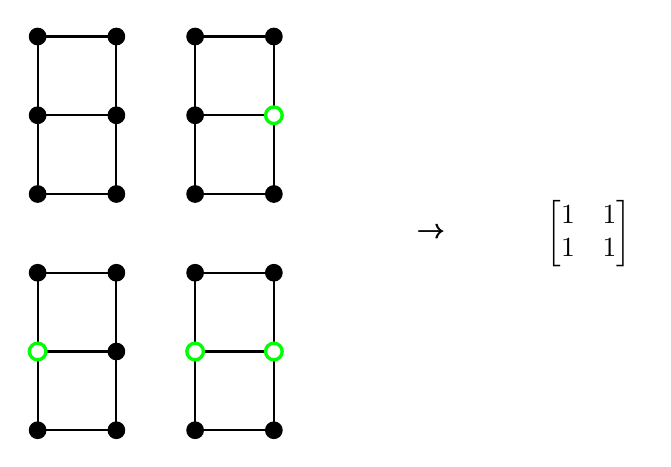
\begin{tikzpicture}
        % row1
        \cell{0}{0}{1}{1}
        \cell{0}{1}{1}{2}

        \cell{2}{0}{3}{1}
        \cell{2}{1}{3}{2}

        % row2
        \cell{0}{3}{1}{4}
        \cell{0}{4}{1}{5}

        \cell{2}{3}{3}{4}
        \cell{2}{4}{3}{5}
        % row 1
        \draw[fill=black] (0,0) circle (3pt);
        \draw[fill=white, draw=green, very thick] (0,1) circle (3pt);
        \draw[fill=black] (0,2) circle (3pt);

        \draw[fill=black] (1,0) circle (3pt);
        \draw[fill=black] (1,1) circle (3pt);
        \draw[fill=black] (1,2) circle (3pt);

        \draw[fill=black] (2,0) circle (3pt);
        \draw[fill=white, draw=green, very thick] (2,1) circle (3pt);
        \draw[fill=black] (2,2) circle (3pt);

        \draw[fill=black] (3,0) circle (3pt);
        \draw[fill=white, draw=green, very thick] (3,1) circle (3pt);
        \draw[fill=black] (3,2) circle (3pt);
        % row 2
        \draw[fill=black] (0,3) circle (3pt);
        \draw[fill=black] (0,4) circle (3pt);
        \draw[fill=black] (0,5) circle (3pt);

        \draw[fill=black] (1,3) circle (3pt);
        \draw[fill=black] (1,4) circle (3pt);
        \draw[fill=black] (1,5) circle (3pt);

        \draw[fill=black] (2,3) circle (3pt);
        \draw[fill=black] (2,4) circle (3pt);
        \draw[fill=black] (2,5) circle (3pt);

        \draw[fill=black] (3,3) circle (3pt);
        \draw[fill=white, draw=green, very thick] (3,4) circle (3pt);
        \draw[fill=black] (3,5) circle (3pt);

        % arrow
        \( \lablnode{5}{2.5}{$\pmb{\to}$} \)
        % matrix
        \( \lablnode{7}{2.5}{$\begin{bmatrix} 1 & 1 \\ 1 & 1 \end{bmatrix}$} \)

    \end{tikzpicture}
\end{center}

If one knows the $A(2)$ weight at, say, position $(0,1)$, then one can identify the mapping by considering appending all possible vertex colorings to the bottom of the column, like so.

\begin{center}
    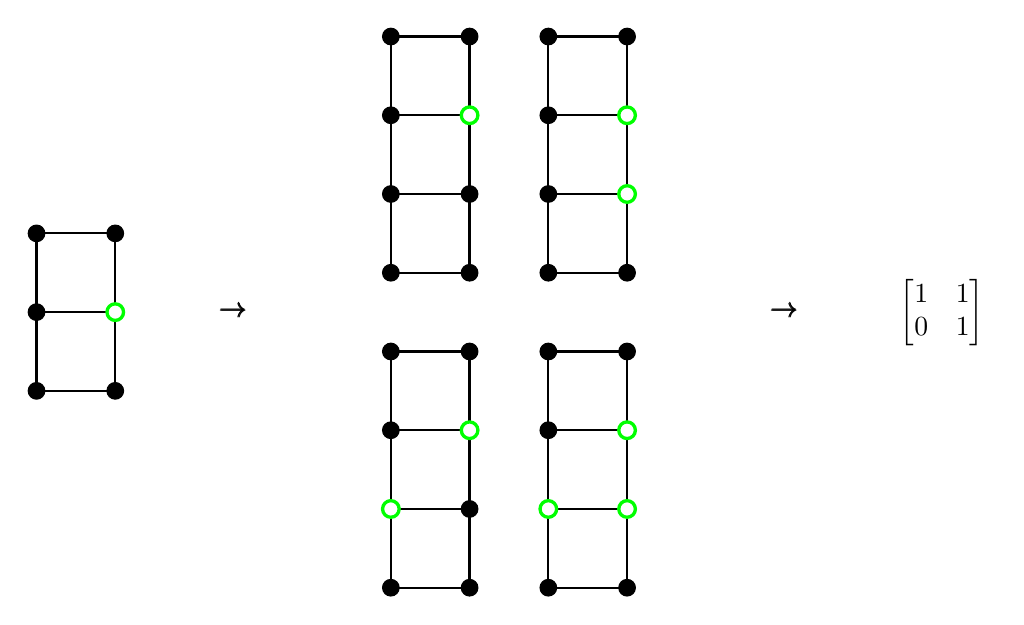
\begin{tikzpicture}
        % row1
        \cell{-4.5}{2.5}{-3.5}{3.5}
        \cell{-4.5}{3.5}{-3.5}{4.5}

        % row 1
        \draw[fill=black] (-4.5,2.5) circle (3pt);
        \draw[fill=black] (-4.5,3.5) circle (3pt);
        \draw[fill=black] (-4.5,4.5) circle (3pt);

        \draw[fill=black] (-3.5,2.5) circle (3pt);
        \draw[fill=white, draw=green, very thick] (-3.5,3.5) circle (3pt);
        \draw[fill=black] (-3.5,4.5) circle (3pt);

        % arrow
        \( \lablnode{-2}{3.5}{$\pmb{\to}$} \)

        % four columns
        \cell{0}{0}{1}{1}
        \cell{0}{1}{1}{2}
        \cell{0}{2}{1}{3}

        \cell{2}{0}{3}{1}
        \cell{2}{1}{3}{2}
        \cell{2}{2}{3}{3}

        \draw[fill=black] (0,0) circle (3pt);
        \draw[fill=white, draw=green, very thick] (0,1) circle (3pt);
        \draw[fill=black] (0,2) circle (3pt);
        \draw[fill=black] (0,3) circle (3pt);

        \draw[fill=black] (1,0) circle (3pt);
        \draw[fill=black] (1,1) circle (3pt);
        \draw[fill=white, draw=green, very thick] (1,2) circle (3pt);
        \draw[fill=black] (1,3) circle (3pt);

        \draw[fill=black] (2,0) circle (3pt);
        \draw[fill=white, draw=green, very thick] (2,1) circle (3pt);
        \draw[fill=black] (2,2) circle (3pt);
        \draw[fill=black] (2,3) circle (3pt);

        \draw[fill=black] (3,0) circle (3pt);
        \draw[fill=white, draw=green, very thick] (3,1) circle (3pt);
        \draw[fill=white, draw=green, very thick] (3,2) circle (3pt);
        \draw[fill=black] (3,3) circle (3pt);

        \cell{0}{4}{1}{5}
        \cell{0}{5}{1}{6}
        \cell{0}{6}{1}{7}

        \cell{2}{4}{3}{5}
        \cell{2}{5}{3}{6}
        \cell{2}{6}{3}{7}

        \draw[fill=black] (0,4) circle (3pt);
        \draw[fill=black] (0,5) circle (3pt);
        \draw[fill=black] (0,6) circle (3pt);
        \draw[fill=black] (0,7) circle (3pt);

        \draw[fill=black] (1,4) circle (3pt);
        \draw[fill=black] (1,5) circle (3pt);
        \draw[fill=white, draw=green, very thick] (1,6) circle (3pt);
        \draw[fill=black] (1,7) circle (3pt);

        \draw[fill=black] (2,4) circle (3pt);
        \draw[fill=black] (2,5) circle (3pt);
        \draw[fill=black] (2,6) circle (3pt);
        \draw[fill=black] (2,7) circle (3pt);

        \draw[fill=black] (3,4) circle (3pt);
        \draw[fill=white, draw=green, very thick] (3,5) circle (3pt);
        \draw[fill=white, draw=green, very thick] (3,6) circle (3pt);
        \draw[fill=black] (3,7) circle (3pt);

        \( \lablnode{5}{3.5}{$\pmb{\to}$} \)

        \( \lablnode{7}{3.5}{$\begin{bmatrix} 1 & 1 \\ 0 & 1 \end{bmatrix}$} \)

    \end{tikzpicture}
\end{center}

If we write $A(2) = \begin{bmatrix}
    1 & 1 \\
    1 & 1 
\end{bmatrix} = 
\begin{bmatrix}
    M_1 & M_2 \\
    M_3 & M_4 
\end{bmatrix}
$, and compute these mappings for all possible parity configurations, we get

$$
A(3) = 
\begin{bmatrix}
    1M_1 & 1M_2 & 1M_1 & 1M_2 \\
    1M_3 & 1M_4 & 0M_3 & 1M_4 \\
    1M_1 & 0M_2 & 1M_1 & 1M_2 \\
    1M_3 & 1M_4 & 1M_3 & 1M_4 \\
\end{bmatrix}.
$$

Finally, as appending any vertex coloring to the bottom of a column only changes the identity of the bottom two sub-colorings, we can write that for any matrix $A(m) =\begin{bmatrix} A_1 & A_2 \\ A_3 & A_4 \end{bmatrix}$ we have 

$$
A(m+1) = 
\begin{bmatrix}
    1M_1 & 1M_2 & 1M_1 & 1M_2 \\
    1M_3 & 1M_4 & 0M_3 & 1M_4 \\
    1M_1 & 0M_2 & 1M_1 & 1M_2 \\
    1M_3 & 1M_4 & 1M_3 & 1M_4 \\
\end{bmatrix},
$$

which completes the proof.

\end{proof}

The method detailed in Theorem \ref{thm: main theorem} generalizes to other tile sets, which we tabularize in Section \ref{section: summary of results} without proof. Interestingly, the method not only generalizes to other tile sets, but can also be augmented to enumerate the more complicated ``messy" polygon mosaics.

\section{Messy Polygon Mosaics}

A \textit{messy polygon mosaic} is a mosaic that contains at least polygon, with no restriction on other shared edges. 

\begin{exmp}
\label{exmp: messy sap}
Below is a messy polygon mosaic of size $(5,7)$ with $1$ polygon hilighted in gray. 

\begin{center}
    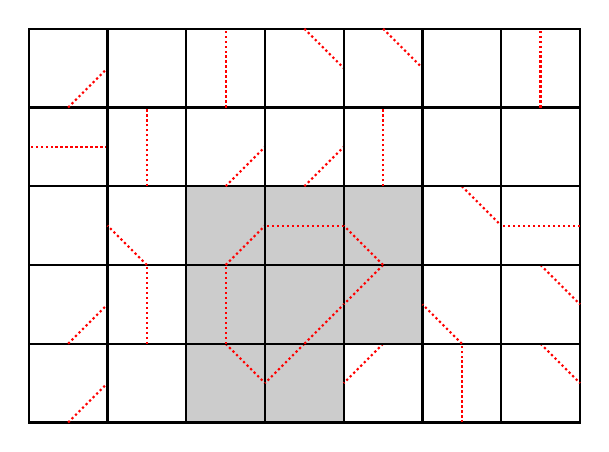
\begin{tikzpicture}
        % row1
        \cellA{0}{0}{1}{1}
        \cell{1}{0}{2}{1}
        \cellDf{2}{0}{3}{1}
        \cellCf{3}{0}{4}{1}
        \cellC{4}{0}{5}{1}
        \cellE{5}{0}{6}{1}
        \cellD{6}{0}{7}{1}
        % row2
        \cellA{0}{1}{1}{2}
        \cellE{1}{1}{2}{2}
        \cellEf{2}{1}{3}{2}
        \cellAf{3}{1}{4}{2}
        \cellCf{4}{1}{5}{2}
        \cellB{5}{1}{6}{2}
        \cellD{6}{1}{7}{2}
        % row3
        \cell{0}{2}{1}{3}
        \cellB{1}{2}{2}{3}
        \cellAf{2}{2}{3}{3}
        \cellFf{3}{2}{4}{3}
        \cellBf{4}{2}{5}{3}
        \cellD{5}{2}{6}{3}
        \cellF{6}{2}{7}{3}
        % row4
        \cellF{0}{3}{1}{4}
        \cellE{1}{3}{2}{4}
        \cellA{2}{3}{3}{4}
        \cellA{3}{3}{4}{4}
        \cellE{4}{3}{5}{4}
        \cell{5}{3}{6}{4}
        \cell{6}{3}{7}{4}
        % row5
        \cellA{0}{4}{1}{5}
        \cell{1}{4}{2}{5}
        \cellE{2}{4}{3}{5}
        \cellD{3}{4}{4}{5}
        \cellD{4}{4}{5}{5}
        \cell{5}{4}{6}{5}
        \cellE{6}{4}{7}{5}
    \end{tikzpicture}
\end{center}
\end{exmp}

Note that one can also consider creating messy polygon mosaics with the alternate tile set below, where the empty tile is removed.

%figure of tiles (colored marknigs!)
\begin{center}
    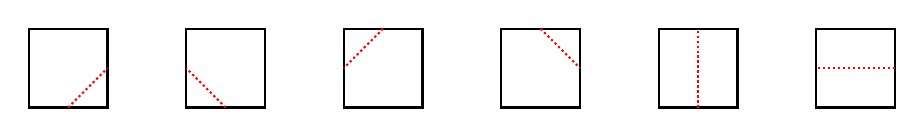
\begin{tikzpicture}
    \cellA{0}{0}{1}{1}
    \cellB{2}{0}{3}{1}
    \cellC{4}{0}{5}{1}
    \cellD{6}{0}{7}{1}
    \cellE{8}{0}{9}{1}
    \cellF{10}{0}{11}{1}    
    \end{tikzpicture}
\end{center}

Due to the fact that the empty tile cannot contribute to the structure of the SAP, enumerating messy polygon mosaics under either tile set can be written with a parameter $b$, where $b=6$ or $b=7$ for the respective tile set. We work with the general $b$ for the remainder of the paper.

Additionally, it turns out that it is easier to enumerate the number of messy mosaics that \textit{do not} contain a SAP. Therefore, let $t_{n,m}$ be the number of mosaics that do not contain a SAP. Clearly $t_{n,m}=t_{m,n}.$ Also from the fact that the smallest SAP is

\begin{center}
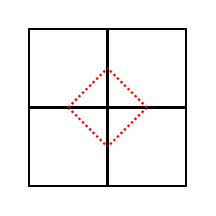
\begin{tikzpicture}
    % row1
    \cellD{0}{0}{1}{1}
    \cellC{1}{0}{2}{1}
    % row2
    \cellA{0}{1}{1}{2}
    \cellB{1}{1}{2}{2}
\end{tikzpicture}
\end{center}

we have that $t_{n,1}=b^n$, and $t_{2,2} = b^4 - 1$. It turns out that using similar techniques to Theorem \ref{thm: main theorem} we can exactly enumerate messy mosaics. 

\begin{thm}
\label{thm: messy mosaics}

Let $
M(2) = \begin{bmatrix}
b^2 & 1 \\
-1 & 1
\end{bmatrix}
$ for $n \geq 2$, where $b = 6$ for the $6$-tile set and $b = 7$ for the $7$-tile set.Then for $m \geq 2$, if
$
M(m) = \begin{bmatrix}
M_1 & M_2 \\
M_3 & M_4
\end{bmatrix},
$ define
$$
M(m+1) = \begin{bmatrix}
bM_1 & bM_2 & \frac{1}{b}M_1 & M_2 \\
bM_3 & bM_4 & 0M_3 & M_4 \\
-\frac{1}{b}M_1 & 0M_2 & \frac{1}{b}M_1 & M_2 \\
M_3 & M_4 & -M_3 & bM_4 \\
\end{bmatrix},
$$

where $M_i$ is a sub-matrix of the block matrix $M(m)$. For the given $m$, define the rows and columns of $M(m)$ as

$$
M(m) = 
\begin{bmatrix}
    r_1 \\
    r_2 \\
    ... \\
    r_{2^{m-1}} \\
\end{bmatrix} =
\begin{bmatrix}
    c_1 & c_2 & ... & c_{2^{m-1}}
\end{bmatrix} 
$$

Then $t_{n,m} = r_1 M(m)^{n-2}c_1 .$
\end{thm}

\section{Proof of Theorem \ref{thm: messy mosaics}}

\begin{proof}
We again consider the parity configurations for a specific $(n,m)$-mosaic. However, there is not a bijection between messy polygon mosaics and parity configurations in the same way as with traditional polygon mosaics. This is because the following cell-parity configurations are no longer uniquely determined.

\begin{center}
    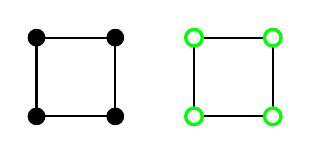
\begin{tikzpicture}
        % row1
        \cell{0}{0}{1}{1}
        \cell{2}{0}{3}{1}

        \draw[fill=black] (0,0) circle (3pt);
        \draw[fill=black] (1,0) circle (3pt);
        \draw[fill=white, draw=green, very thick] (2,0) circle (3pt);
        \draw[fill=white, draw=green, very thick] (3,0) circle (3pt);

        \draw[fill=black] (0,1) circle (3pt);
        \draw[fill=black] (1,1) circle (3pt);
        \draw[fill=white, draw=green, very thick] (2,1) circle (3pt);
        \draw[fill=white, draw=green, very thick] (3,1) circle (3pt);
        
    \end{tikzpicture}
\end{center}

Additionally, the sub parity configurations shown below

\begin{center}
    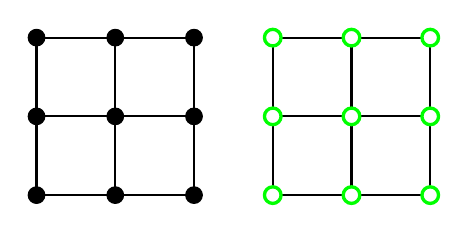
\begin{tikzpicture}
        % row1
        \cell{0}{0}{1}{1}
        \cell{0}{1}{1}{2}
        \cell{1}{0}{2}{1}
        \cell{1}{1}{2}{2}

        \draw[fill=black] (0,0) circle (3pt);
        \draw[fill=black] (1,0) circle (3pt);
        \draw[fill=black] (2,0) circle (3pt);

        \draw[fill=black] (0,1) circle (3pt);
        \draw[fill=black] (1,1) circle (3pt);
        \draw[fill=black] (2,1) circle (3pt);

        \draw[fill=black] (0,2) circle (3pt);
        \draw[fill=black] (1,2) circle (3pt);
        \draw[fill=black] (2,2) circle (3pt);
        % row1
        \cell{3}{0}{4}{1}
        \cell{3}{1}{4}{2}
        \cell{4}{0}{5}{1}
        \cell{4}{1}{5}{2}

        \draw[fill=white, draw=green, very thick] (3,0) circle (3pt);
        \draw[fill=white, draw=green, very thick] (4,0) circle (3pt);
        \draw[fill=white, draw=green, very thick] (5,0) circle (3pt);

        \draw[fill=white, draw=green, very thick] (3,1) circle (3pt);
        \draw[fill=white, draw=green, very thick] (4,1) circle (3pt);
        \draw[fill=white, draw=green, very thick] (5,1) circle (3pt);

        \draw[fill=white, draw=green, very thick] (3,2) circle (3pt);
        \draw[fill=white, draw=green, very thick] (4,2) circle (3pt);
        \draw[fill=white, draw=green, very thick] (5,2) circle (3pt);
    \end{tikzpicture}
\end{center}

are now ambiguous as to whether or not they represent a SAP. Critically, both of the following parity configurations could include the right-most messy polygon mosaic. 

\begin{center}
    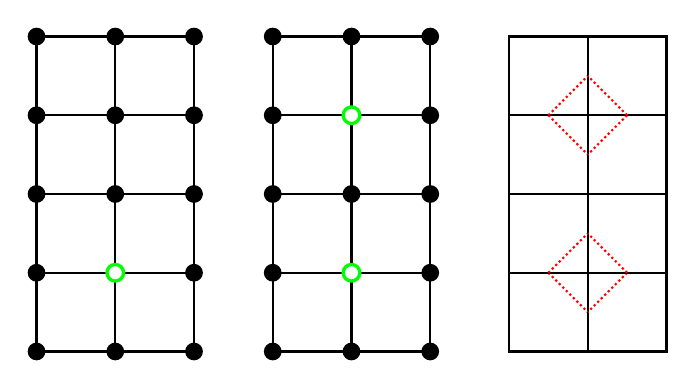
\begin{tikzpicture}
        % row1
        \cell{0}{0}{1}{1}
        \cell{0}{1}{1}{2}
        \cell{0}{2}{1}{3}
        \cell{0}{3}{1}{4}
        \cell{1}{0}{2}{1}
        \cell{1}{1}{2}{2}
        \cell{1}{2}{2}{3}
        \cell{1}{3}{2}{4}
        

        \draw[fill=black] (0,0) circle (3pt);
        \draw[fill=black] (1,0) circle (3pt);
        \draw[fill=black] (2,0) circle (3pt);

        \draw[fill=black] (0,1) circle (3pt);
        \draw[fill=white, draw=green, very thick] (1,1) circle (3pt);
        \draw[fill=black] (2,1) circle (3pt);

        \draw[fill=black] (0,2) circle (3pt);
        \draw[fill=black] (1,2) circle (3pt);
        \draw[fill=black] (2,2) circle (3pt);

        \draw[fill=black] (0,3) circle (3pt);
        \draw[fill=black] (1,3) circle (3pt);
        \draw[fill=black] (2,3) circle (3pt);

        \draw[fill=black] (0,4) circle (3pt);
        \draw[fill=black] (1,4) circle (3pt);
        \draw[fill=black] (2,4) circle (3pt);

        % row1
        \cell{3}{0}{4}{1}
        \cell{3}{1}{4}{2}
        \cell{3}{2}{4}{3}
        \cell{3}{3}{4}{4}
        \cell{4}{0}{5}{1}
        \cell{4}{1}{5}{2}
        \cell{4}{2}{5}{3}
        \cell{4}{3}{5}{4}
        

        \draw[fill=black] (3,0) circle (3pt);
        \draw[fill=black] (4,0) circle (3pt);
        \draw[fill=black] (5,0) circle (3pt);

        \draw[fill=black] (3,1) circle (3pt);
        \draw[fill=white, draw=green, very thick] (4,1) circle (3pt);
        \draw[fill=black] (5,1) circle (3pt);

        \draw[fill=black] (3,2) circle (3pt);
        \draw[fill=black] (4,2) circle (3pt);
        \draw[fill=black] (5,2) circle (3pt);

        \draw[fill=black] (3,3) circle (3pt);
        \draw[fill=white, draw=green, very thick] (4,3) circle (3pt);
        \draw[fill=black] (5,3) circle (3pt);

        \draw[fill=black] (3,4) circle (3pt);
        \draw[fill=black] (4,4) circle (3pt);
        \draw[fill=black] (5,4) circle (3pt);


        \cellD{6}{0}{7}{1}
        \cellC{7}{0}{8}{1}

        \cellA{6}{1}{7}{2}
        \cellB{7}{1}{8}{2}

        \cellD{6}{2}{7}{3}
        \cellC{7}{2}{8}{3}    

        \cellA{6}{3}{7}{4}
        \cellB{7}{3}{8}{4}    

    \end{tikzpicture}
\end{center}

In fact, the number of SAPs that appear in a given messy polygon mosaic is exactly the number of parity configurations that map to that mosaic. Therefore, if we are to count these mosaics, we need to account for this double-counting with the inclusion-exclusion principle.  

To create an analagous result to Theorem \ref{thm: main theorem} we need to find a weight assignment to the $16$ parity configurations below that fulfill a set of conditions.

\begin{center}
    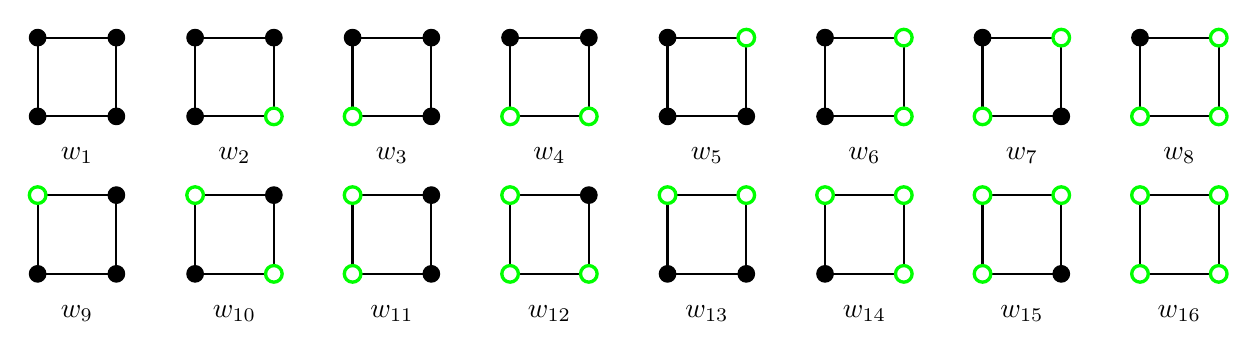
\begin{tikzpicture}
        % row1
        \cell{0}{0}{1}{1}
        \cell{2}{0}{3}{1}
        \cell{4}{0}{5}{1}
        \cell{6}{0}{7}{1}
        \cell{8}{0}{9}{1}
        \cell{10}{0}{11}{1}
        \cell{12}{0}{13}{1}
        \cell{14}{0}{15}{1}
        % row2
        \cell{0}{2}{1}{3}
        \cell{2}{2}{3}{3}This means that
        \cell{4}{2}{5}{3}
        \cell{6}{2}{7}{3}
        \cell{8}{2}{9}{3}
        \cell{10}{2}{11}{3}
        \cell{12}{2}{13}{3}
        \cell{14}{2}{15}{3}
        % label for row1
        \draw[fill=black] (0,0) circle (3pt);
        \draw[fill=black] (1,0) circle (3pt);
        \draw[fill=black] (2,0) circle (3pt);
        \draw[fill=white, draw=green, very thick] (3,0) circle (3pt);
        \draw[fill=white, draw=green, very thick] (4,0) circle (3pt);
        \draw[fill=black] (5,0) circle (3pt);
        \draw[fill=white, draw=green, very thick] (6,0) circle (3pt);
        \draw[fill=white, draw=green, very thick] (7,0) circle (3pt);
        \draw[fill=black] (8,0) circle (3pt);
        \draw[fill=black] (9,0) circle (3pt);
        \draw[fill=black] (10,0) circle (3pt);
        \draw[fill=white, draw=green, very thick] (11,0) circle (3pt);
        \draw[fill=white, draw=green, very thick] (12,0) circle (3pt);
        \draw[fill=black] (13,0) circle (3pt);
        \draw[fill=white, draw=green, very thick] (14,0) circle (3pt);
        \draw[fill=white, draw=green, very thick] (15,0) circle (3pt);
        % label for row1
        \draw[fill=white, draw=green, very thick] (0,1) circle (3pt);
        \draw[fill=black] (1,1) circle (3pt);
        \draw[fill=white, draw=green, very thick] (2,1) circle (3pt);
        \draw[fill=black] (3,1) circle (3pt);
        \draw[fill=white, draw=green, very thick] (4,1) circle (3pt);
        \draw[fill=black] (5,1) circle (3pt);
        \draw[fill=white, draw=green, very thick] (6,1) circle (3pt);
        \draw[fill=black] (7,1) circle (3pt);
        \draw[fill=white, draw=green, very thick] (8,1) circle (3pt);
        \draw[fill=white, draw=green, very thick] (9,1) circle (3pt);
        \draw[fill=white, draw=green, very thick] (10,1) circle (3pt);
        \draw[fill=white, draw=green, very thick] (11,1) circle (3pt);
        \draw[fill=white, draw=green, very thick] (12,1) circle (3pt);
        \draw[fill=white, draw=green, very thick] (13,1) circle (3pt);
        \draw[fill=white, draw=green, very thick] (14,1) circle (3pt);
        \draw[fill=white, draw=green, very thick] (15,1) circle (3pt);
        % label for row1
        \draw[fill=black] (0,2) circle (3pt);
        \draw[fill=black] (1,2) circle (3pt);
        \draw[fill=black] (2,2) circle (3pt);
        \draw[fill=white, draw=green, very thick] (3,2) circle (3pt);
        \draw[fill=white, draw=green, very thick] (4,2) circle (3pt);
        \draw[fill=black] (5,2) circle (3pt);
        \draw[fill=white, draw=green, very thick] (6,2) circle (3pt);
        \draw[fill=white, draw=green, very thick] (7,2) circle (3pt);
        \draw[fill=black] (8,2) circle (3pt);
        \draw[fill=black] (9,2) circle (3pt);
        \draw[fill=black] (10,2) circle (3pt);
        \draw[fill=white, draw=green, very thick] (11,2) circle (3pt);
        \draw[fill=white, draw=green, very thick] (12,2) circle (3pt);
        \draw[fill=black] (13,2) circle (3pt);
        \draw[fill=white, draw=green, very thick] (14,2) circle (3pt);
        \draw[fill=white, draw=green, very thick] (15,2) circle (3pt);
        % label for row1
        \draw[fill=black] (0,3) circle (3pt);
        \draw[fill=black] (1,3) circle (3pt);
        \draw[fill=black] (2,3) circle (3pt);
        \draw[fill=black] (3,3) circle (3pt);
        \draw[fill=black] (4,3) circle (3pt);
        \draw[fill=black] (5,3) circle (3pt);
        \draw[fill=black] (6,3) circle (3pt);
        \draw[fill=black] (7,3) circle (3pt);
        \draw[fill=black] (8,3) circle (3pt);
        \draw[fill=white, draw=green, very thick] (9,3) circle (3pt);
        \draw[fill=black] (10,3) circle (3pt);
        \draw[fill=white, draw=green, very thick] (11,3) circle (3pt);
        \draw[fill=black] (12,3) circle (3pt);
        \draw[fill=white, draw=green, very thick] (13,3) circle (3pt);
        \draw[fill=black] (14,3) circle (3pt);
        \draw[fill=white, draw=green, very thick] (15,3) circle (3pt);
        % numbers row 1
        \( \lablnode{0.5}{-0.5}{$w_{9}$} \)
        \( \lablnode{2.5}{-0.5}{$w_{10}$} \)
        \( \lablnode{4.5}{-0.5}{$w_{11}$} \)
        \( \lablnode{6.5}{-0.5}{$w_{12}$} \)
        \( \lablnode{8.5}{-0.5}{$w_{13}$} \)
        \( \lablnode{10.5}{-0.5}{$w_{14}$} \)
        \( \lablnode{12.5}{-0.5}{$w_{15}$} \)
        \( \lablnode{14.5}{-0.5}{$w_{16}$} \)
        % numbers row 2
        \( \lablnode{0.5}{1.5}{$w_{1}$} \)
        \( \lablnode{2.5}{1.5}{$w_{2}$} \)
        \( \lablnode{4.5}{1.5}{$w_{3}$} \)
        \( \lablnode{6.5}{1.5}{$w_{4}$} \)
        \( \lablnode{8.5}{1.5}{$w_{5}$} \)
        \( \lablnode{10.5}{1.5}{$w_{6}$} \)
        \( \lablnode{12.5}{1.5}{$w_{7}$} \)
        \( \lablnode{14.5}{1.5}{$w_{8}$} \)
    \end{tikzpicture}
\end{center}

First $w_{7}=w_{10}=0$, as again these are impossible parity configurations for our tile set. Next notice that $w_{1} = w_{16} = b$, as these cells do not indicate a specific tile.  The remaining weights uniquely specify a tile, and so are equal to $1$ or $-1$. But how do we find these assignments?

First notice that we want a weight assignment so that the parity configurations for a given SAP multiply to $-1$. This is due to the inclusion-exclusion principle. This means that if there are multiple SAPs in a mosaic, then the product will be positive if there is an even number of SAPs specified, and negative if there is an odd number specified.

Next note the following lemma.
\begin{lemma}
    \label{lemma: build bigger saps}
    One can construct all larger SAPs from the smallest SAP using a finite set of transformations $S$.
\end{lemma}

\begin{proof}
    TODO
\end{proof}

This is because one can find $w_{1} , \dots, w_{16}$ so that the following two constraints hold:

\begin{constraint}
    \label{constraint: smallest sap prod}
    The weights associated with the smallest SAP multiply to $-1$, ie. $w_2 w_3 w_5 w_9 = -1.$ 
\end{constraint}

\begin{constraint}
    \label{constraint: prod works}
    \emph{All} transformations in $S$ preserve the weight product of a changed SAP.
\end{constraint}

Constraint \ref{constraint: smallest sap prod} and Constraint \ref{constraint: prod works} amount to a series of constraints on the values of $w_i$. The derivation for these constraints can be found in the Appendix. Choosing a solution set from these constraints gives the following weights.

\begin{center}
    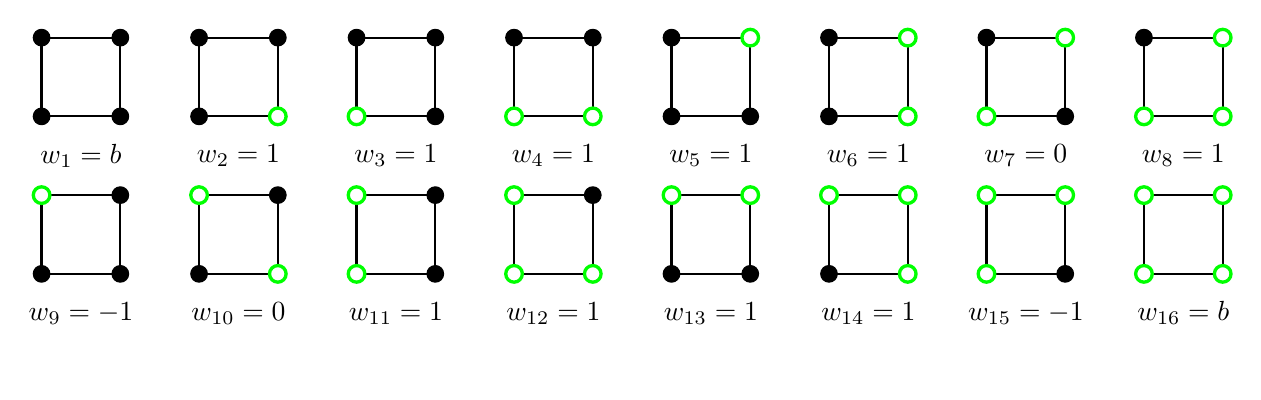
\begin{tikzpicture}
        % row1
        \cell{0}{0}{1}{1}
        \cell{2}{0}{3}{1}
        \cell{4}{0}{5}{1}
        \cell{6}{0}{7}{1}
        \cell{8}{0}{9}{1}
        \cell{10}{0}{11}{1}
        \cell{12}{0}{13}{1}
        \cell{14}{0}{15}{1}
        % row2
        \cell{0}{2}{1}{3}
        \cell{2}{2}{3}{3}
        \cell{4}{2}{5}{3}
        \cell{6}{2}{7}{3}
        \cell{8}{2}{9}{3}
        \cell{10}{2}{11}{3}
        \cell{12}{2}{13}{3}
        \cell{14}{2}{15}{3}
        % label for row1
        \draw[fill=black] (0,0) circle (3pt);
        \draw[fill=black] (1,0) circle (3pt);
        \draw[fill=black] (2,0) circle (3pt);
        \draw[fill=white, draw=green, very thick] (3,0) circle (3pt);
        \draw[fill=white, draw=green, very thick] (4,0) circle (3pt);
        \draw[fill=black] (5,0) circle (3pt);
        \draw[fill=white, draw=green, very thick] (6,0) circle (3pt);
        \draw[fill=white, draw=green, very thick] (7,0) circle (3pt);
        \draw[fill=black] (8,0) circle (3pt);
        \draw[fill=black] (9,0) circle (3pt);
        \draw[fill=black] (10,0) circle (3pt);
        \draw[fill=white, draw=green, very thick] (11,0) circle (3pt);
        \draw[fill=white, draw=green, very thick] (12,0) circle (3pt);
        \draw[fill=black] (13,0) circle (3pt);
        \draw[fill=white, draw=green, very thick] (14,0) circle (3pt);
        \draw[fill=white, draw=green, very thick] (15,0) circle (3pt);
        % label for row1
        \draw[fill=white, draw=green, very thick] (0,1) circle (3pt);
        \draw[fill=black] (1,1) circle (3pt);
        \draw[fill=white, draw=green, very thick] (2,1) circle (3pt);
        \draw[fill=black] (3,1) circle (3pt);
        \draw[fill=white, draw=green, very thick] (4,1) circle (3pt);
        \draw[fill=black] (5,1) circle (3pt);
        \draw[fill=white, draw=green, very thick] (6,1) circle (3pt);
        \draw[fill=black] (7,1) circle (3pt);
        \draw[fill=white, draw=green, very thick] (8,1) circle (3pt);
        \draw[fill=white, draw=green, very thick] (9,1) circle (3pt);
        \draw[fill=white, draw=green, very thick] (10,1) circle (3pt);
        \draw[fill=white, draw=green, very thick] (11,1) circle (3pt);
        \draw[fill=white, draw=green, very thick] (12,1) circle (3pt);
        \draw[fill=white, draw=green, very thick] (13,1) circle (3pt);
        \draw[fill=white, draw=green, very thick] (14,1) circle (3pt);
        \draw[fill=white, draw=green, very thick] (15,1) circle (3pt);
        % label for row1
        \draw[fill=black] (0,2) circle (3pt);
        \draw[fill=black] (1,2) circle (3pt);
        \draw[fill=black] (2,2) circle (3pt);
        \draw[fill=white, draw=green, very thick] (3,2) circle (3pt);
        \draw[fill=white, draw=green, very thick] (4,2) circle (3pt);
        \draw[fill=black] (5,2) circle (3pt);
        \draw[fill=white, draw=green, very thick] (6,2) circle (3pt);
        \draw[fill=white, draw=green, very thick] (7,2) circle (3pt);
        \draw[fill=black] (8,2) circle (3pt);
        \draw[fill=black] (9,2) circle (3pt);
        \draw[fill=black] (10,2) circle (3pt);
        \draw[fill=white, draw=green, very thick] (11,2) circle (3pt);
        \draw[fill=white, draw=green, very thick] (12,2) circle (3pt);
        \draw[fill=black] (13,2) circle (3pt);
        \draw[fill=white, draw=green, very thick] (14,2) circle (3pt);
        \draw[fill=white, draw=green, very thick] (15,2) circle (3pt);
        % label for row1
        \draw[fill=black] (0,3) circle (3pt);
        \draw[fill=black] (1,3) circle (3pt);
        \draw[fill=black] (2,3) circle (3pt);
        \draw[fill=black] (3,3) circle (3pt);
        \draw[fill=black] (4,3) circle (3pt);
        \draw[fill=black] (5,3) circle (3pt);
        \draw[fill=black] (6,3) circle (3pt);
        \draw[fill=black] (7,3) circle (3pt);
        \draw[fill=black] (8,3) circle (3pt);
        \draw[fill=white, draw=green, very thick] (9,3) circle (3pt);
        \draw[fill=black] (10,3) circle (3pt);
        \draw[fill=white, draw=green, very thick] (11,3) circle (3pt);
        \draw[fill=black] (12,3) circle (3pt);
        \draw[fill=white, draw=green, very thick] (13,3) circle (3pt);
        \draw[fill=black] (14,3) circle (3pt);
        \draw[fill=white, draw=green, very thick] (15,3) circle (3pt);
        % numbers row 1
        \( \lablnode{0.5}{-0.5}{$w_{9}=-1$} \)
        \( \lablnode{2.5}{-0.5}{$w_{10}=0$} \)
        \( \lablnode{4.5}{-0.5}{$w_{11}=1$} \)
        \( \lablnode{6.5}{-0.5}{$w_{12}=1$} \)
        \( \lablnode{8.5}{-0.5}{$w_{13}=1$} \)
        \( \lablnode{10.5}{-0.5}{$w_{14}=1$} \)
        \( \lablnode{12.5}{-0.5}{$w_{15}=-1$} \)
        \( \lablnode{14.5}{-0.5}{$w_{16}=b$} \)
        % numbers row 2
        \( \lablnode{0.5}{1.5}{$w_{1}=b$} \)
        \( \lablnode{2.5}{1.5}{$w_{2}=1$} \)
        \( \lablnode{4.5}{1.5}{$w_{3}=1$} \)
        \( \lablnode{6.5}{1.5}{$w_{4}=1$} \)
        \( \lablnode{8.5}{1.5}{$w_{5}=1$} \)
        \( \lablnode{10.5}{1.5}{$w_{6}=1$} \)
        \( \lablnode{12.5}{1.5}{$w_{7}=0$} \)
        \( \lablnode{14.5}{1.5}{$w_{8}=1$} \)
    \end{tikzpicture}
\end{center}

This immediately gives us a way to construct an analagous definition for our transition matrixes $M(m) = \begin{bmatrix} M_1 & M_2 \\ M_3 & M_4 \end{bmatrix}$. As the appending of a cell parity configuration can possibly change the number of admitted cells, we define $v_{1} ,\dots, v_{16}$ for the associated change in the number of mosaics for the recursive definition of $M(m+1)$. A simple way to obtain $v_{1} ,\dots, v_{16}$ is to directly compute $M(2)$ and $M(3)$ and compare their values like so.

$$M(2) = 
\begin{bmatrix}
    b^2 & 1 \\
    -1 & 1
\end{bmatrix}, M(3)=
\begin{bmatrix}
b^3 & b & b & 1 \\
-b & b & 0 & 1 \\
-b & 0 & b & 1 \\
-1 & 1 & 1 & b \\
\end{bmatrix}.$$

This gives

$$
M(m+1) = 
\begin{bmatrix}
    v_{1}M_1 & v_{2}M_2 & v_{3}M_1 & v_{4}M_2 \\
    v_{5}M_3 & v_{6}M_4 & v_{7}M_3 & v_{8}M_4 \\
    v_{9}M_1 & v_{10}M_2 & v_{11}M_1 & v_{12}M_2 \\
    v_{13}M_3 & v_{14}M_4 & v_{15}M_3 & v_{16}M_4 \\
\end{bmatrix} =
\begin{bmatrix}
bM_1 & bM_2 & \frac{1}{b}M_1 & M_2 \\
bM_3 & bM_4 & 0M_3 & M_4 \\
-\frac{1}{b}M_1 & 0M_2 & \frac{1}{b}M_1 & M_2 \\
M_3 & M_4 & -M_3 & bM_4 \\
\end{bmatrix}.
$$

An analagous argument to Theorem \ref{thm: main theorem} gives the result.

\end{proof}

% \begin{theorem}
%     \label{thm: growth rate}    
%     Let the probability that an $(n,m)$-mosaic \textit{does not} contain a SAP be denoted $p_{n,m} = \frac{t_{n,m}}{7^{nm}}$. Then the growth rate of the main diagonal $p_{n,n}$ has
%     $$\gamma = \lim_{n \to \infty} \frac{p_{n+1,n+1}p_{n-1,n-1}}{p_{n,n}^2} = ?$$
% \end{theorem}

\section{Appendix}

Flipping the parity of a single vertex in a parity configuration changes the $4$ surrounding cells. This creates a constraint on a subset of $w_1 ,\dots, w_{16}.$ 

The flipping of parity of a single vertex can result in $2$ distinct types of constraints. Let a constraint of \textit{Type 1} be a parity flip that does not change the number of SAPs in the parity configuration. For example, consider the following flip of the center vertex in the following portion of a parity configuration.

\begin{center}
    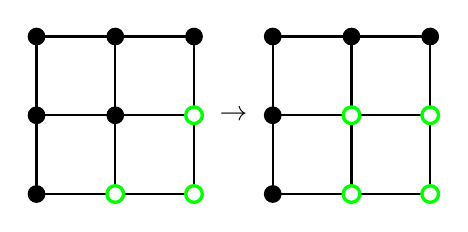
\begin{tikzpicture}
        % row1
        \cell{0}{0}{1}{1}
        \cell{1}{0}{2}{1}
        % row2
        \cell{0}{1}{1}{2}
        \cell{1}{1}{2}{2}
        % label for row1
        \draw[fill=black] (0,0) circle (3pt);
        \draw[fill=white, draw=green, very thick] (1,0) circle (3pt);
        \draw[fill=white, draw=green, very thick] (2,0) circle (3pt);
        % label for row2
        \draw[fill=black] (0,1) circle (3pt);
        \draw[fill=black] (1,1) circle (3pt);
        \draw[fill=white, draw=green, very thick] (2,1) circle (3pt);
        % label for row3
        \draw[fill=black] (0,2) circle (3pt);
        \draw[fill=black] (1,2) circle (3pt);
        \draw[fill=black] (2,2) circle (3pt);
        % row1
        \cell{3}{0}{4}{1}
        \cell{4}{0}{5}{1}
        % row2
        \cell{3}{1}{4}{2}
        \cell{4}{1}{5}{2}
        % label for row1
        \draw[fill=black] (3,0) circle (3pt);
        \draw[fill=white, draw=green, very thick] (4,0) circle (3pt);
        \draw[fill=white, draw=green, very thick] (5,0) circle (3pt);
        % label for row2
        \draw[fill=black] (3,1) circle (3pt);
        \draw[fill=white, draw=green, very thick] (4,1) circle (3pt);
        \draw[fill=white, draw=green, very thick] (5,1) circle (3pt);
        % label for row3
        \draw[fill=black] (3,2) circle (3pt);
        \draw[fill=black] (4,2) circle (3pt);
        \draw[fill=black] (5,2) circle (3pt);

        \( \lablnode{2.5}{1}{$\rightarrow$} \)
    \end{tikzpicture}
\end{center}

As this does not change the associated number of SAPs in the larger parity configuration, we want this to preserve the sign of the weight product. This gives the following associated constraint. 

$$\text{sign}(w_{1}w_{2}w_{5}w_{9}) = \text{sign}(w_{2}w_{4}w_{6}w_{16}).$$

Now let a constraint of \textit{Type 2} be a parity flip that does change the number of SAPs. For example, consider flipping the center vertex of the following portion of a parity configuration.

\begin{center}
    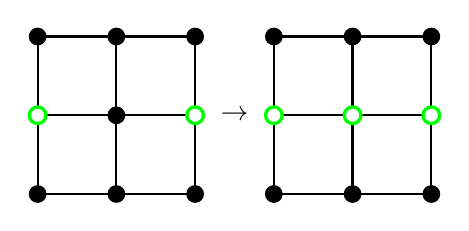
\begin{tikzpicture}
        % row1
        \cell{0}{0}{1}{1}
        \cell{1}{0}{2}{1}
        % row2
        \cell{0}{1}{1}{2}
        \cell{1}{1}{2}{2}
        % label for row1
        \draw[fill=black] (0,0) circle (3pt);
        \draw[fill=black] (1,0) circle (3pt);
        \draw[fill=black] (2,0) circle (3pt);
        % label for row2
        \draw[fill=white, draw=green, very thick] (0,1) circle (3pt);
        \draw[fill=black] (1,1) circle (3pt);
        \draw[fill=white, draw=green, very thick] (2,1) circle (3pt);
        % label for row3
        \draw[fill=black] (0,2) circle (3pt);
        \draw[fill=black] (1,2) circle (3pt);
        \draw[fill=black] (2,2) circle (3pt);
        % row1
        \cell{3}{0}{4}{1}
        \cell{4}{0}{5}{1}
        % row2
        \cell{3}{1}{4}{2}
        \cell{4}{1}{5}{2}
        % label for row1
        \draw[fill=black] (3,0) circle (3pt);
        \draw[fill=black] (4,0) circle (3pt);
        \draw[fill=black] (5,0) circle (3pt);
        % label for row2
        \draw[fill=white, draw=green, very thick] (3,1) circle (3pt);
        \draw[fill=white, draw=green, very thick] (4,1) circle (3pt);
        \draw[fill=white, draw=green, very thick] (5,1) circle (3pt);
        % label for row3
        \draw[fill=black] (3,2) circle (3pt);
        \draw[fill=black] (4,2) circle (3pt);
        \draw[fill=black] (5,2) circle (3pt);

        \( \lablnode{2.5}{1}{$\rightarrow$} \)
    \end{tikzpicture}
\end{center}

The above transformation corresponds with \textit{either} two distinct SAPs joining into one SAP \textit{or} one SAP splitting into two distinct SAPs. In either case, we want the sign of the product to switch. This corresponds with the following constraint.

$$\text{sign}(w_{3}w_{2}w_{9}w_{5}) = -\text{sign}(w_{4}w_{4}w_{13}w_{13}).$$

All Type 1 constraints are as follows. For the following set of equations, assume the equals sign ($=$) means \textit{only} equal in sign.

\begin{eqnarray*}
    w_{1}w_{1}w_{2}w_{3} = w_{2}w_{3}w_{6}w_{11} & w_{1}w_{1}w_{2}w_{4} = w_{2}w_{3}w_{6}w_{12} & w_{1}w_{1}w_{4}w_{3} = w_{2}w_{3}w_{8}w_{11} \\
    w_{1}w_{1}w_{4}w_{4} = w_{2}w_{3}w_{8}w_{12} & w_{1}w_{2}w_{1}w_{5} = w_{2}w_{4}w_{5}w_{13} & w_{1}w_{2}w_{1}w_{6} = w_{2}w_{4}w_{5}w_{14} \\
    w_{1}w_{2}w_{2}w_{8} = w_{2}w_{4}w_{6}w_{16} & w_{1}w_{2}w_{4}w_{8} = w_{2}w_{4}w_{8}w_{16} & w_{3}w_{1}w_{9}w_{1} = w_{4}w_{3}w_{13}w_{9} \\
    w_{3}w_{1}w_{11}w_{1} = w_{4}w_{3}w_{15}w_{9} & w_{3}w_{1}w_{12}w_{3} = w_{4}w_{3}w_{16}w_{11} & w_{3}w_{1}w_{12}w_{4} = w_{4}w_{3}w_{16}w_{12} \\
    w_{3}w_{2}w_{12}w_{8} = w_{4}w_{4}w_{16}w_{16} & w_{1}w_{6}w_{1}w_{5} = w_{2}w_{8}w_{5}w_{13} & w_{1}w_{6}w_{1}w_{6} = w_{2}w_{8}w_{5}w_{14} \\
    w_{1}w_{6}w_{2}w_{8} = w_{2}w_{8}w_{6}w_{16} & w_{1}w_{6}w_{4}w_{8} = w_{2}w_{8}w_{8}w_{16} & w_{3}w_{6}w_{12}w_{8} = w_{4}w_{8}w_{16}w_{16} \\
    w_{5}w_{9}w_{1}w_{1} = w_{6}w_{11}w_{5}w_{9} & w_{5}w_{13}w_{1}w_{1} = w_{6}w_{15}w_{5}w_{9} & w_{5}w_{14}w_{1}w_{5} = w_{6}w_{16}w_{5}w_{13} \\
    w_{5}w_{14}w_{1}w_{6} = w_{6}w_{16}w_{5}w_{14} & w_{5}w_{14}w_{2}w_{8} = w_{6}w_{16}w_{6}w_{16} & w_{5}w_{14}w_{4}w_{8} = w_{6}w_{16}w_{8}w_{16} \\
    w_{11}w_{1}w_{9}w_{1} = w_{12}w_{3}w_{13}w_{9} & w_{11}w_{1}w_{11}w_{1} = w_{12}w_{3}w_{15}w_{9} & w_{11}w_{1}w_{12}w_{3} = w_{12}w_{3}w_{16}w_{11} \\
    w_{11}w_{1}w_{12}w_{4} = w_{12}w_{3}w_{16}w_{12} & w_{11}w_{2}w_{12}w_{8} = w_{12}w_{4}w_{16}w_{16} & w_{11}w_{6}w_{12}w_{8} = w_{12}w_{8}w_{16}w_{16} \\
    w_{13}w_{9}w_{1}w_{1} = w_{14}w_{11}w_{5}w_{9} & w_{15}w_{9}w_{9}w_{1} = w_{16}w_{11}w_{13}w_{9} & w_{15}w_{9}w_{11}w_{1} = w_{16}w_{11}w_{15}w_{9} \\
    w_{15}w_{9}w_{12}w_{3} = w_{16}w_{11}w_{16}w_{11} & w_{15}w_{9}w_{12}w_{4} = w_{16}w_{11}w_{16}w_{12} & w_{13}w_{13}w_{1}w_{1} = w_{14}w_{15}w_{5}w_{9} \\
    w_{13}w_{14}w_{1}w_{5} = w_{14}w_{16}w_{5}w_{13} & w_{13}w_{14}w_{1}w_{6} = w_{14}w_{16}w_{5}w_{14} & w_{13}w_{14}w_{2}w_{8} = w_{14}w_{16}w_{6}w_{16} \\
    w_{13}w_{14}w_{4}w_{8} = w_{14}w_{16}w_{8}w_{16} & w_{15}w_{13}w_{9}w_{1} = w_{16}w_{15}w_{13}w_{9} & w_{15}w_{13}w_{11}w_{1} = w_{16}w_{15}w_{15}w_{9} \\
    w_{15}w_{13}w_{12}w_{3} = w_{16}w_{15}w_{16}w_{11} & w_{15}w_{13}w_{12}w_{4} = w_{16}w_{15}w_{16}w_{12} & w_{15}w_{14}w_{9}w_{5} = w_{16}w_{16}w_{13}w_{13} \\
    w_{15}w_{14}w_{9}w_{6} = w_{16}w_{16}w_{13}w_{14} & w_{15}w_{14}w_{11}w_{5} = w_{16}w_{16}w_{15}w_{13} & w_{15}w_{14}w_{11}w_{6} = w_{16}w_{16}w_{15}w_{14} \\
\end{eqnarray*}

Similarly, all Type 2 constraints are as follows. Again, for the following set of equations, assume the equals sign ($=$) means \textit{only} equal in sign.

\begin{eqnarray*}
        -w_{3}w_{2}w_{9}w_{5} = w_{4}w_{4}w_{13}w_{13} & -w_{3}w_{2}w_{9}w_{6} = w_{4}w_{4}w_{13}w_{14} & -w_{3}w_{2}w_{11}w_{5} = w_{4}w_{4}w_{15}w_{13} \\
        -w_{3}w_{2}w_{11}w_{6} = w_{4}w_{4}w_{15}w_{14} & -w_{3}w_{6}w_{9}w_{5} = w_{4}w_{8}w_{13}w_{13} & -w_{3}w_{6}w_{9}w_{6} = w_{4}w_{8}w_{13}w_{14} \\
        -w_{3}w_{6}w_{11}w_{5} = w_{4}w_{8}w_{15}w_{13} & -w_{3}w_{6}w_{11}w_{6} = w_{4}w_{8}w_{15}w_{14} & -w_{5}w_{9}w_{2}w_{3} = w_{6}w_{11}w_{6}w_{11} \\
        -w_{5}w_{9}w_{2}w_{4} = w_{6}w_{11}w_{6}w_{12} & -w_{5}w_{9}w_{4}w_{3} = w_{6}w_{11}w_{8}w_{11} & -w_{5}w_{9}w_{4}w_{4} = w_{6}w_{11}w_{8}w_{12} \\
        -w_{5}w_{13}w_{2}w_{3} = w_{6}w_{15}w_{6}w_{11} & -w_{5}w_{13}w_{2}w_{4} = w_{6}w_{15}w_{6}w_{12} & -w_{5}w_{13}w_{4}w_{3} = w_{6}w_{15}w_{8}w_{11} \\
        -w_{5}w_{13}w_{4}w_{4} = w_{6}w_{15}w_{8}w_{12} & -w_{11}w_{2}w_{9}w_{5} = w_{12}w_{4}w_{13}w_{13} & -w_{11}w_{2}w_{9}w_{6} = w_{12}w_{4}w_{13}w_{14} \\
        -w_{11}w_{2}w_{11}w_{5} = w_{12}w_{4}w_{15}w_{13} & -w_{11}w_{2}w_{11}w_{6} = w_{12}w_{4}w_{15}w_{14} & -w_{11}w_{6}w_{9}w_{5} = w_{12}w_{8}w_{13}w_{13} \\
        -w_{11}w_{6}w_{9}w_{6} = w_{12}w_{8}w_{13}w_{14} & -w_{11}w_{6}w_{11}w_{5} = w_{12}w_{8}w_{15}w_{13} & -w_{11}w_{6}w_{11}w_{6} = w_{12}w_{8}w_{15}w_{14} \\
        -w_{13}w_{9}w_{2}w_{3} = w_{14}w_{11}w_{6}w_{11} & -w_{13}w_{9}w_{2}w_{4} = w_{14}w_{11}w_{6}w_{12} & -w_{13}w_{9}w_{4}w_{3} = w_{14}w_{11}w_{8}w_{11} \\
        -w_{13}w_{9}w_{4}w_{4} = w_{14}w_{11}w_{8}w_{12} & -w_{13}w_{13}w_{2}w_{3} = w_{14}w_{15}w_{6}w_{11} & -w_{13}w_{13}w_{2}w_{4} = w_{14}w_{15}w_{6}w_{12} \\
        -w_{13}w_{13}w_{4}w_{3} = w_{14}w_{15}w_{8}w_{11} & -w_{13}w_{13}w_{4}w_{4} = w_{14}w_{15}w_{8}w_{12} & 
\end{eqnarray*}

Solving all Type 1 and Type 2 constraints gives the following solution set.

\begin{center}
\begin{tabular}{|c|c|c|c|c|c|c|c|c|c|c|c|c|c|c|c|} 
\hline
$w_{1}$ & $w_{2}$ & $w_{3}$ & $w_{4}$ & $w_{5}$ & $w_{6}$ & $w_{7}$ & $w_{8}$ & $w_{9}$ & $w_{10}$ & $w_{11}$ & $w_{12}$ & $w_{13}$ & $w_{14}$ & $w_{15}$ & $w_{16}$ \\
\hline
b & -1 & -1 & -1 & -1 & -1 & 0 & -1 & 1 & 0 & -1 & -1 & -1 & -1 & 1 & b \\
b & -1 & -1 & -1 & -1 & 1 & 0 & 1 & 1 & 0 & 1 & 1 & -1 & 1 & -1 & b \\
b & -1 & -1 & -1 & 1 & -1 & 0 & -1 & -1 & 0 & -1 & -1 & -1 & 1 & -1 & b \\
b & -1 & -1 & -1 & 1 & 1 & 0 & 1 & -1 & 0 & 1 & 1 & -1 & -1 & 1 & b \\
b & -1 & -1 & 1 & -1 & -1 & 0 & 1 & 1 & 0 & -1 & 1 & 1 & 1 & -1 & b \\
b & -1 & -1 & 1 & -1 & 1 & 0 & -1 & 1 & 0 & 1 & -1 & 1 & -1 & 1 & b \\
b & -1 & -1 & 1 & 1 & -1 & 0 & 1 & -1 & 0 & -1 & 1 & 1 & -1 & 1 & b \\
b & -1 & -1 & 1 & 1 & 1 & 0 & -1 & -1 & 0 & 1 & -1 & 1 & 1 & -1 & b \\
b & -1 & 1 & -1 & -1 & -1 & 0 & -1 & -1 & 0 & -1 & 1 & -1 & -1 & -1 & b \\
b & -1 & 1 & -1 & -1 & 1 & 0 & 1 & -1 & 0 & 1 & -1 & -1 & 1 & 1 & b \\
b & -1 & 1 & -1 & 1 & -1 & 0 & -1 & 1 & 0 & -1 & 1 & -1 & 1 & 1 & b \\
b & -1 & 1 & -1 & 1 & 1 & 0 & 1 & 1 & 0 & 1 & -1 & -1 & -1 & -1 & b \\
b & -1 & 1 & 1 & -1 & -1 & 0 & 1 & -1 & 0 & -1 & -1 & 1 & 1 & 1 & b \\
b & -1 & 1 & 1 & -1 & 1 & 0 & -1 & -1 & 0 & 1 & 1 & 1 & -1 & -1 & b \\
b & -1 & 1 & 1 & 1 & -1 & 0 & 1 & 1 & 0 & -1 & -1 & 1 & -1 & -1 & b \\
b & -1 & 1 & 1 & 1 & 1 & 0 & -1 & 1 & 0 & 1 & 1 & 1 & 1 & 1 & b \\
b & 1 & -1 & -1 & -1 & -1 & 0 & 1 & -1 & 0 & -1 & -1 & -1 & -1 & -1 & b \\
b & 1 & -1 & -1 & -1 & 1 & 0 & -1 & -1 & 0 & 1 & 1 & -1 & 1 & 1 & b \\
b & 1 & -1 & -1 & 1 & -1 & 0 & 1 & 1 & 0 & -1 & -1 & -1 & 1 & 1 & b \\
b & 1 & -1 & -1 & 1 & 1 & 0 & -1 & 1 & 0 & 1 & 1 & -1 & -1 & -1 & b \\
b & 1 & -1 & 1 & -1 & -1 & 0 & -1 & -1 & 0 & -1 & 1 & 1 & 1 & 1 & b \\
b & 1 & -1 & 1 & -1 & 1 & 0 & 1 & -1 & 0 & 1 & -1 & 1 & -1 & -1 & b \\
b & 1 & -1 & 1 & 1 & -1 & 0 & -1 & 1 & 0 & -1 & 1 & 1 & -1 & -1 & b \\
b & 1 & -1 & 1 & 1 & 1 & 0 & 1 & 1 & 0 & 1 & -1 & 1 & 1 & 1 & b \\
b & 1 & 1 & -1 & -1 & -1 & 0 & 1 & 1 & 0 & -1 & 1 & -1 & -1 & 1 & b \\
b & 1 & 1 & -1 & -1 & 1 & 0 & -1 & 1 & 0 & 1 & -1 & -1 & 1 & -1 & b \\
b & 1 & 1 & -1 & 1 & -1 & 0 & 1 & -1 & 0 & -1 & 1 & -1 & 1 & -1 & b \\
b & 1 & 1 & -1 & 1 & 1 & 0 & -1 & -1 & 0 & 1 & -1 & -1 & -1 & 1 & b \\
b & 1 & 1 & 1 & -1 & -1 & 0 & -1 & 1 & 0 & -1 & -1 & 1 & 1 & -1 & b \\
b & 1 & 1 & 1 & -1 & 1 & 0 & 1 & 1 & 0 & 1 & 1 & 1 & -1 & 1 & b \\
b & 1 & 1 & 1 & 1 & -1 & 0 & -1 & -1 & 0 & -1 & -1 & 1 & -1 & 1 & b \\
b & 1 & 1 & 1 & 1 & 1 & 0 & 1 & -1 & 0 & 1 & 1 & 1 & 1 & -1 & b \\
\hline
\end{tabular}
\end{center}

Any of these assignments are sufficient for calculating $t_{n,m}$. 

\section{Summary of Results}
\label{section: summary of results}

TODO make table with tile sets and matrices

\printbibliography

\end{document}